%%%%%%%%%%%%%%%%%%%%%%%%%%%%%%
\chapter{Phase I upgrade of the CMS pixel barrel detector}
\label{ch:Phase1Intro}
%%%%%%%%%%%%%%%%%%%%%%%%%%%%%%

The present pixel detector will be replaced with a new pixel system in order to maintain the excellent tracking performance of CMS with the upcoming higher luminosity conditions at the LHC.
This project is referred to as ``Phase I pixel upgrade'' and it was defined in 2012~\cite{Dominguez:1481838}. The new upgraded detector comprises four barrel layers and three forward disks to provide on average one more spatial point measurement per track compared to the present system, in the whole detector acceptance range. It also provides improved track impact parameter resolution reducing the radius of the innermost layer and increasing radial acceptance. 
Further improvement is obtained thanks to optimized engineering of the mechanical design and services of the detector, that provide a substantial reduction of the passive material in the tracking volume despite the addition of one barrel layer. Since the innermost sensitive layer is closer to the interaction point compared to the current detector, faster front-end electronics has been developed to operate with high hit efficiency and low dead-time.
%Details on the main features of the new barrel pixel system will be given in the following.
In this chapter, the main features of the new barrel pixel system are introduced.\\
%This chapter provides a description of the main features of the new barrel pixel system.

During LS1 eight prototype Phase-1 pixel modules were installed in the CMS detector, on the third unpopulated disk. This so-called pilot system was commissioned and integrated into the central DAQ and control system, and took data in 2015--2016, with the aim of gaining operation experience under realistic conditions.

As for the current barrel pixel detector, the supply tubes have been assembled and tested at the University of Zurich, while the modules have been mounted on the detector mechanical structure at PSI. The integration of the supply tubes with the detector is currently ongoing and the installation into CMS and commissioning of the complete system is planned for March 2017.

Several procedures for testing the new system have been developed over the last three years, thanks to a test stand assembled at the University of Zurich. The test stand, described in this chapter, includes a slice of the CMS pixel data-acquisition system and all components of the upgraded read out chain, together with a number of detector modules. It allowed for detailed evaluation and verification of the components placed on the supply tubes before their integration.
I have contributed to the assembly of the test system and I implemented some of its functionalities. Furthermore, I employed the system to test a new calibration procedure that I developed in POS. The aim of the procedure is to guarantee a check out of the detector functionalities during assembly and commissioning. This work, detailed in the following, has been crucial to gain experience with the new barrel pixel system and to understand the changes that had to be applied to the software to be able to operate with it.

%%%%%%%%%%%%%%%%%%%%%%%%%%%%%%
\section{Motivations}
%%%%%%%%%%%%%%%%%%%%%%%%%%%%%%

The proposed upgrade of the CMS pixel detector aims at maintaining the excellent performance of the current detector up to and beyond an instantaneous luminosity of $2\times10^{34}\percms$ and a pileup of 50.
The limitations of the current detector for increasing luminosity and pileup can be seen in Fig.~\ref{fig:PixEff}, which shows the hit efficiency for the various layers of the current pixel detector in collisions during 2016.
The leading effect is a dynamic data loss in the readout chip which increases with instantaneous luminosity and trigger rate. This loss of data depends on both the occupancy and trigger rates and comes primarily from two sources, buffer size and readout speed. Between L1 triggers pixel hits are stored in a finite sized buffer before being readout at the next L1 trigger, if this buffer is full the ROC cannot record any more hits and subsequent hits are lost. When a L1 triggers the readout, double columns that are being read out are blocked from having hits recorded and the buffer is cleared after the readout; thus, data can be lost if the readout is slow or the L1 trigger rate is high.
Simulation studies showed that for an instantaneous luminosity of $2\times10^{34}\percms$ and a bunch crossing time of 25\unit{ns} (50\unit{ns}),
the expected dynamic inefficiency for the current pixel detector increases up to 15\% (50\%) for ROCs in the first barrel layer.
The track reconstruction efficiency is also affected by the finite size of the buffers on the readout chip. This effect can be seen in Fig.~\ref{fig:trackEffPix}, which shows the track reconstruction efficiency for muons coming from the Z boson decay as a function of the number of primary vertices, as measured in 2016 data with a T\&P method. The efficiency is high and well described in the simulation, but slowly degrades as the number of pileup events increases.
A new ROC for the upgrade pixel detector will largely reduce these effects.\\

\begin{figure}[!htb]
 \begin{center}
 \subfigure[]{\label{fig:PixEff_a}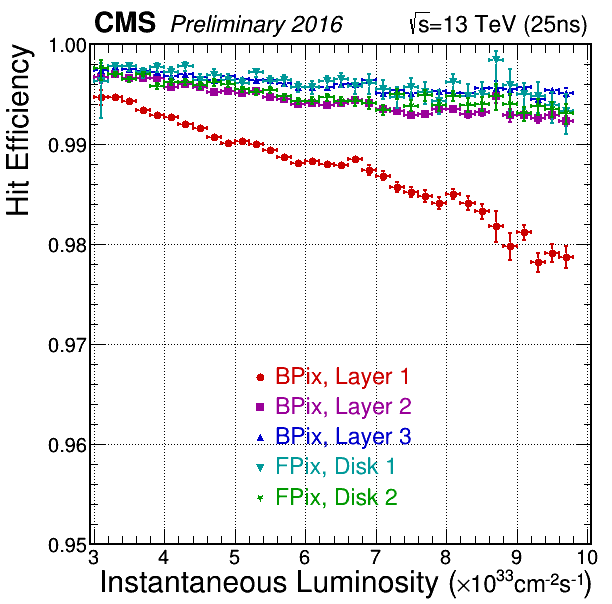
\includegraphics[width=0.45\textwidth]{\chsixteen/HitEfficiency_vs_InstLumi_LayersDisks_2016Data.png}}
 \subfigure[]{\label{fig:PixEff_b}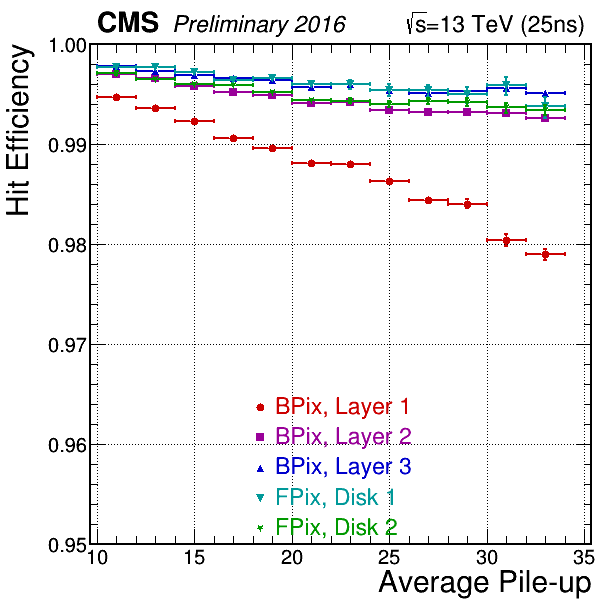
\includegraphics[width=0.45\textwidth]{\chsixteen/HitEfficiency_vs_Pileup_LayersDisks_2016Data.png}}
 \end{center}
 \caption{Hit efficiency for the various layers of the current pixel detector for 2016 collisions as a function of (a) the instantaneous luminosity and (b) the average number of inelastic pp collisions~\cite{PixelOffline}.}
 \label{fig:PixEff}
\end{figure}

Further effects contributing to inefficiencies in the track reconstruction arise from failures in the tracking algorithms for events with a large number of hits. In fact, with more interactions per crossing giving rise to additional hits in the tracking detectors, the pattern recognition becomes more difficult. Under these conditions, the CPU time required for tracking largely increases in both the HLT and offline processing. In addition, keeping the same level of tracking efficiency results in a higher level of fake tracks; alternatively, the tracking can be tuned for lower fake rate at the expense of reduced efficiency.
In order to keep both the CPU time and fake rate under control for luminosities of $2\times10^{34}\percms$, the tracking has to be tuned to have generally lower efficiency that at lower luminosities. This is obtained requiring hits in 3 pixel barrel layers. With an extra pixel layer negative effects of pileup can be partly mitigated.\\

Degradation in the performance of the current detector are further due to radiation damage resulting in reduced charge collection and hence, in degradation of hit detection efficiency and resolution.
Although the degradation can initially be mitigated mostly with increase in voltage, and modification of the pixel cluster hit templates, eventually the reduced collected charge cannot be compensated. The hit efficiency is expected to be less affected but the reduced charge sharing and eventual breaking up of clusters will degrade the hit resolution. Although the upgrade pixel sensor would suffer similar radiation damage, such effects can be compensated by a much lower charge threshold for the new readout chip. This improvement would largely mitigates the effects of reduced collected charge, so degradation in hit resolution should be much reduced comparing to the same radiation fluence.\\

The passive material in the tracking volume is known to lead to tracking inefficiencies.
In particular, a significant portion of material is present in the region near $|\eta| = 1.5$ where the bulkhead with services from BPix meets the FPix.
This material also contribute to additional complications for track pattern recognition in a high pileup environment.
The upgrade pixel detector, even with an extra layer features less passive material in the tracking volume, due to a new lightweight construction, cooling, and relocation of passive material out of the tracking region.

Details on the new detector layout and front-end electronics are given in the next chapter.

\begin{figure}[!htb]
 \begin{center}
 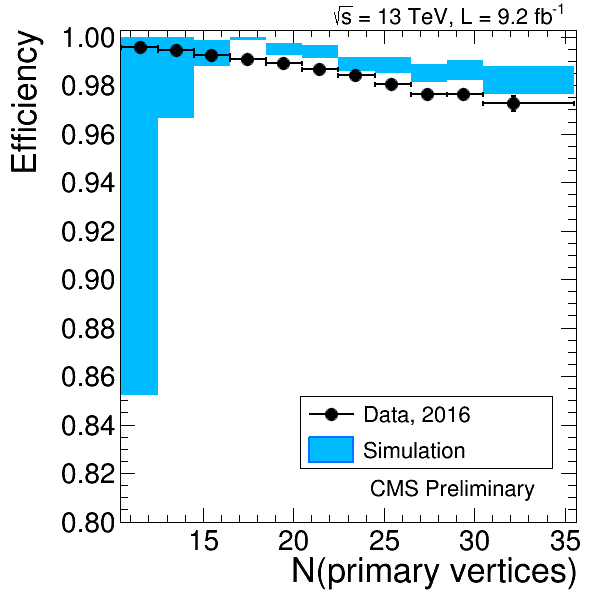
\includegraphics[width=0.45\textwidth]{\chsixteen/eff_vtx_dr030e030_corr.png}
 \end{center}
 \caption{Track reconstruction efficiency for 2016 data and simulation for muons coming from the Z decay as a function of the number of primary vertices~\cite{TrkCMSPublicResults}.}
 \label{fig:trackEffPix}
\end{figure}

%%%%%%%%%%%%%%%%%%%%%%%%%%%%%%
\section{Detector layout}
%%%%%%%%%%%%%%%%%%%%%%%%%%%%%%

The proposed upgraded pixel detector consists of four barrel layers and three disk on either side of the interaction point. The layout of the upgrade pixel system is compared to the current pixel system in Fig.~\ref{fig:Phase1Layout}.
The barrel layers have a length of 548.8 mm and are placed at radii of 30, 68, 109, and 160\mm. Compared to the present BPix, there is one new layer at high radius.
The radius of the innermost layer is reduced by 10\mm while layers 2 and 3 are almost unchanged. 

\begin{figure}[!htb]
 \begin{center}
 \subfigure[]{\label{fig:Phase1Layout_a}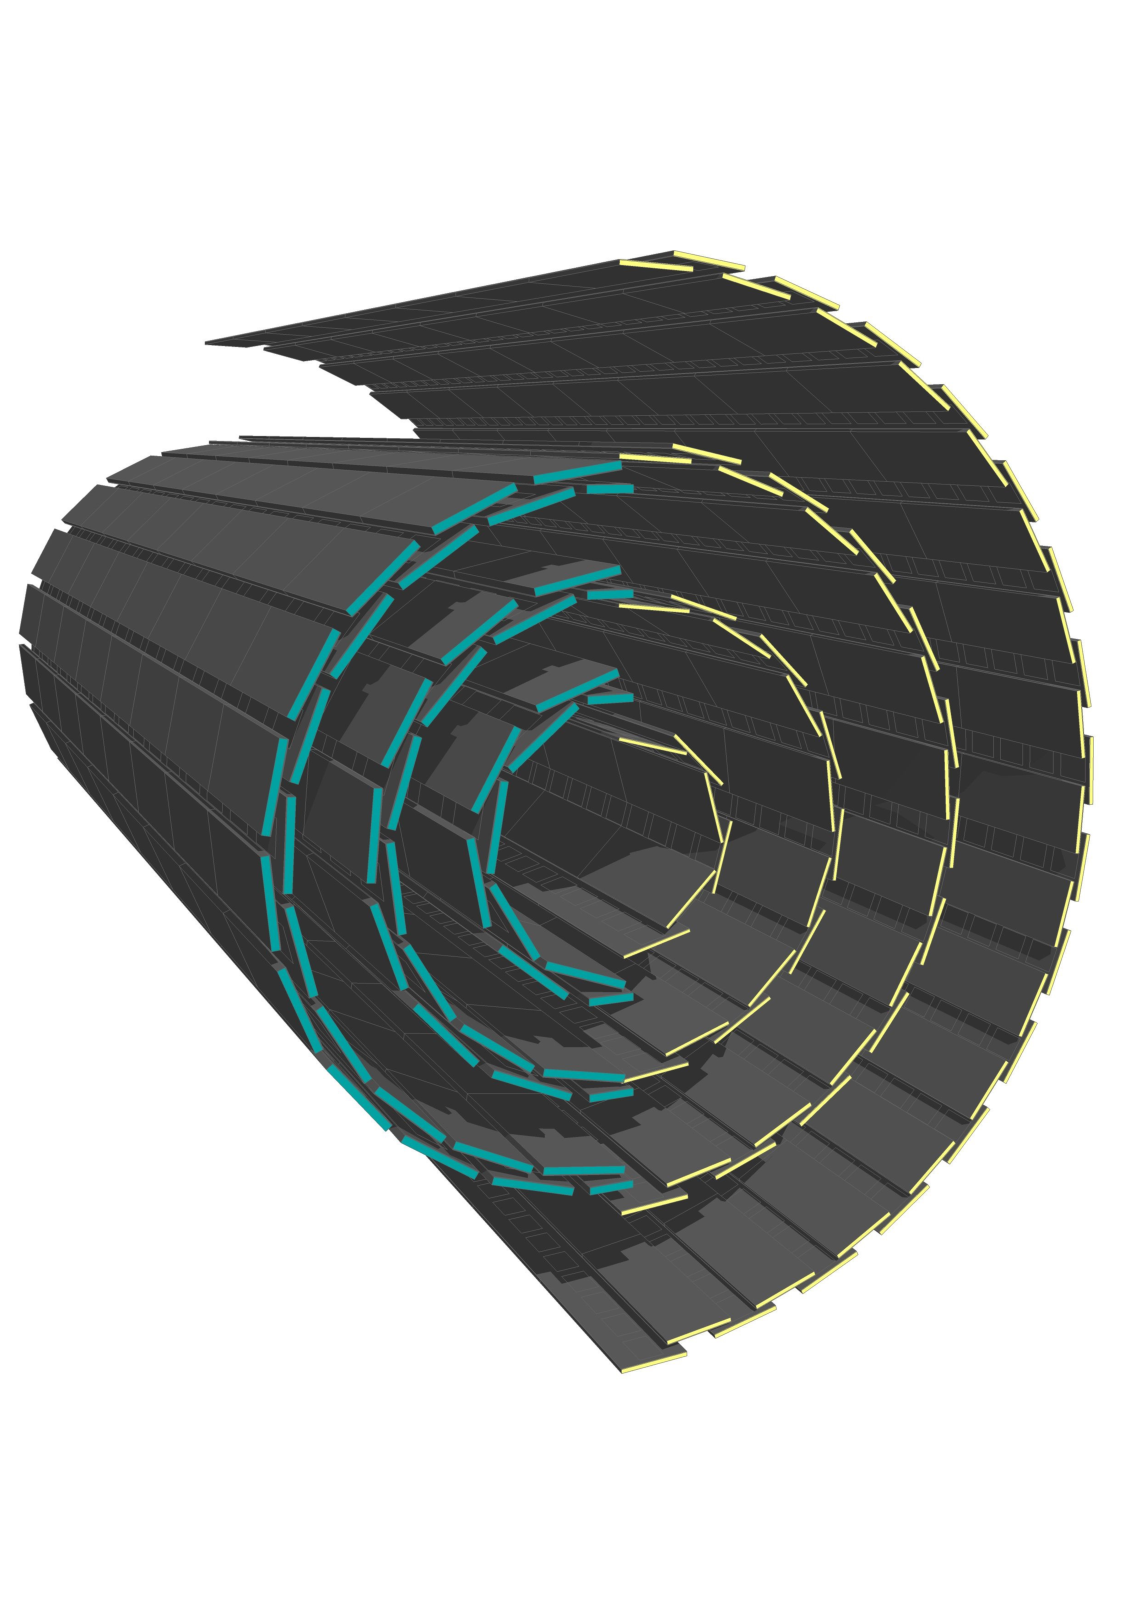
\includegraphics[width=0.26\textwidth]{\chsixteen/phase0-vs-phase1-3D.pdf}}\hspace{0.2cm}
 \subfigure[]{\label{fig:Phase1Layout_b}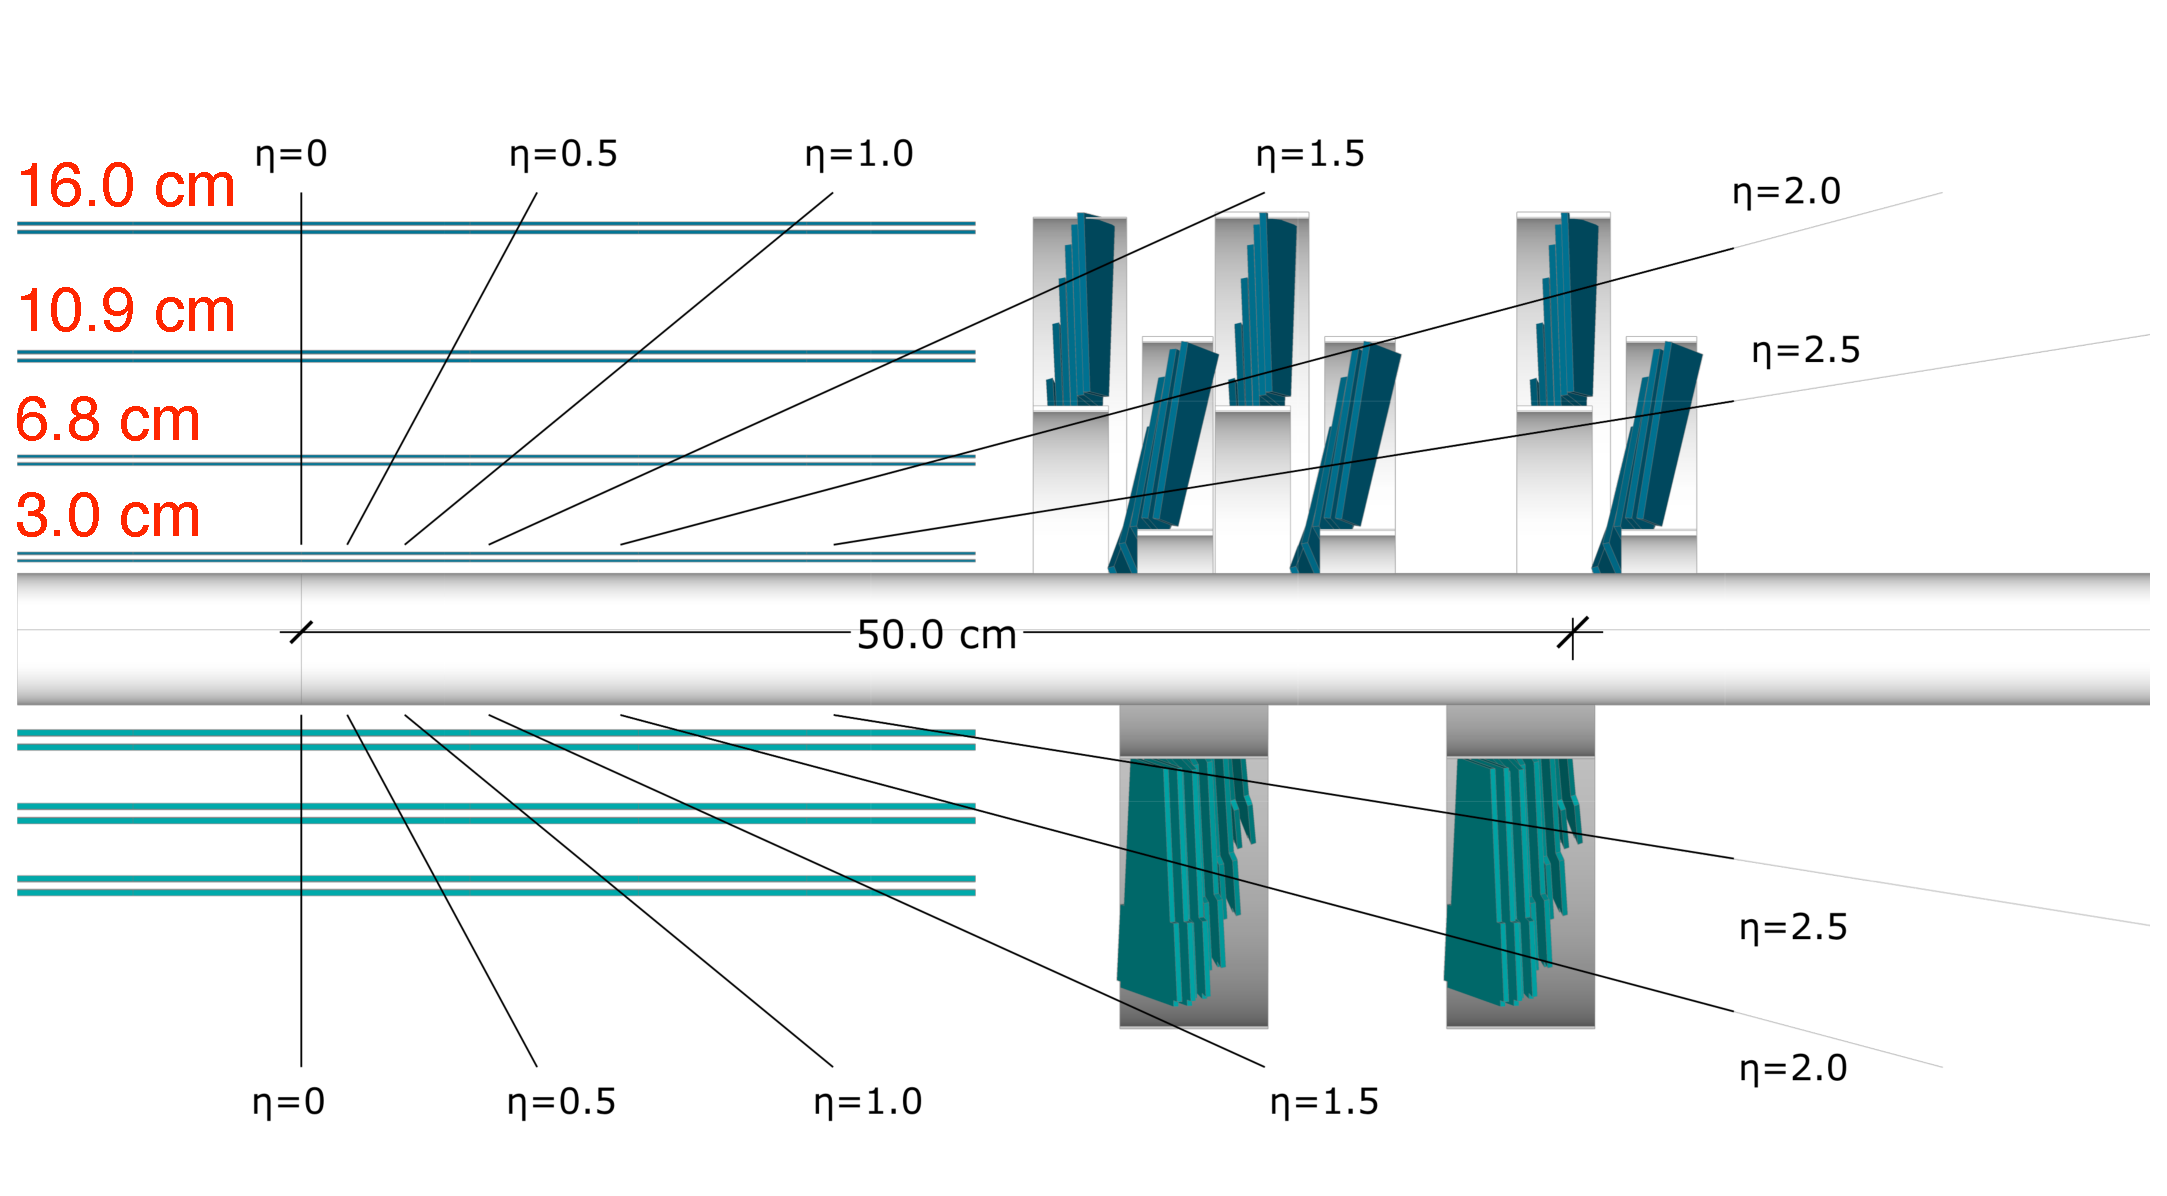
\includegraphics[width=0.65\textwidth]{\chsixteen/phase0-vs-phase1-layout.pdf}}
 \end{center}
 \caption{(a) Layout of the proposed upgraded pixel detector compared to the current detector layout in longitudinal view. (b) Three-dimensional view of the upgraded and current BPix detectors.}
 \label{fig:Phase1Layout}
\end{figure}

The total number of BPix modules will increase to 1,184 compared to 768 modules in the present detector, with an increase in the pixel count from 48 million to 79 million.
The modules are mounted on lightweight mechanical structures built from carbon fiber.
The modules design and composition is almost equal in the whole pixel detector, except for the innermost layer where a considerable higher data rate is expected.
Furthermore half modules are no longer used to join the two halves, while a slightly more complex design of the mechanical support structure enables the use of full modules throughout.
The pixel detector modules will be described in more details in the next section.

The cooling pipes diameter is significantly reduced with respect to the present detector thanks to the usage of a two-phase CO$_2$ cooling system which requires a much smaller mass flow than C$_6$F$_{14}$.
This reduces substantially the amount of material in the tracking region. A further, significant reduction is achieved by moving the module connector area from the detector bulkheads to higher $z$, outside of the tracker acceptance, by using longer and more flexible module cables. As a replacement, micro twisted pair cables made of copper are used. They have a diameter of only 127\mum and are able to transmit the 400\unit{Mbit/s} readout signal. Multiple twisted pairs are used to transmit the different signals, including clock, I$^2$C, trigger, data, etc. Power is conducted in parallel through multiple copper clad aluminium wires with a diameter of 90\mum. Signal and power cables are braided into a single strand. They are about 95\unit{cm} in length for all modules. Each wire of the strand is soldered onto a custom made board that fits into a commercial connector. The connector on the module side is soldered to the HDI.
The obtained reduction in the material budget can bee seen in Fig.~\ref{fig:Phase1Budget}, which shows a comparison of the radiation length and nuclear interaction length of the present and upgrade pixel detectors as a function of $\eta$.

\begin{figure}[!htb]
 \begin{center}
 \subfigure[]{\label{fig:Phase1Budget_a}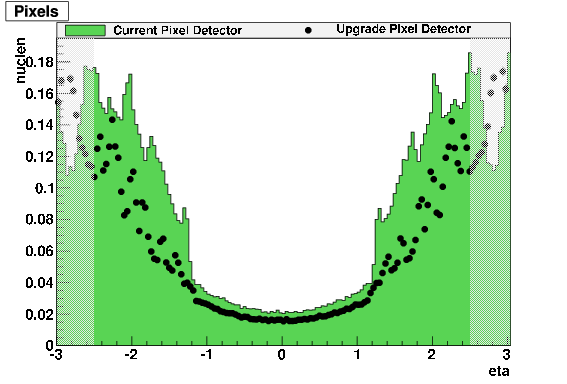
\includegraphics[width=0.45\textwidth]{\chsixteen/ch2_PIX_leta_428r30.png}}
 \subfigure[]{\label{fig:Phase1Budget_b}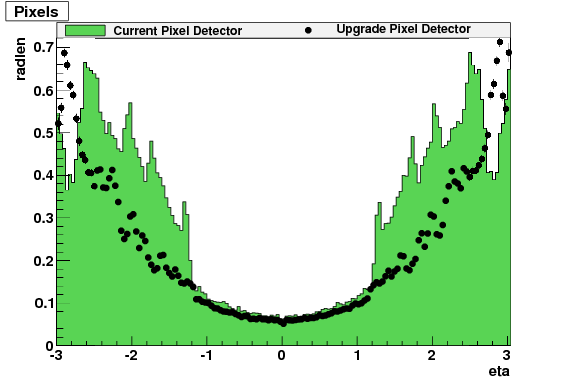
\includegraphics[width=0.45\textwidth]{\chsixteen/ch2_PIX_xeta_428r30.png}}
 \end{center}
 \caption{Material budget in the pixel detector shown in units of radiation length (a), and in units of nuclear interaction length (b) as a function of $\eta$; this is given for the current (green histogram) and upgraded (black points) pixel detector. The shaded region at high $\eta$ is outside the region for track reconstruction~\cite{Dominguez:1481838}.}
 \label{fig:Phase1Budget}
\end{figure}

The overall layout of the system is unchanged. The detector barrel is complemented with four supply tubes on the $+z$ and $-z$ sides. The supply tubes carry electrical connections and cooling lines from the patch panels to the barrel bulkheads, and house auxiliary front-end electronics. However, the upgrade system has to fit in the same mechanical envelope as the current system and reuse existing services, power cables and optical fibers. This puts strong constraints on the design of the new system. In particular, higher bandwidth electronics is need. Since the upgrade detector has 1.9 times more channels than the current detector, the power consumption increases accordingly. The upgrade system uses DC-DC power converters~\cite{1748-0221-10-01-C01052} to supply the necessary current to the modules while reusing the existing infrastructure.

%%%%%%%%%%%%%%%%%%%%%%%%%%%%%%
\section{Pixel modules}
%%%%%%%%%%%%%%%%%%%%%%%%%%%%%%

The pixel modules for the upgrade are of similar configuration compared to the ones employed in the present detector. The main changes concern the design of the ROCs and the TBMs as described in the following.
Fig.~\ref{fig:Phase1Mod} shows a drawing of the pixel module employed for the outer barrel layers.
The innermost barrel layer features a different ROC that allows to cope with even more extreme conditions at such small radii, while its modules differ mostly by the way they are mounted and by the cables used.
%Modules of the other parts of the detector differ mostly by the way they are mounted and by the cables used.
From top to bottom, the figure shows the cables with a connector print, the HDI with the TBM mounted in the center, the silicon pixel sensor, $2\times8$ ROCs and base strips for mounting.

The sensor used in the upgrade is the same technology as the one used in the current detector. For the innermost layer, where the close proximity to the interaction point leads to the highest radiation damage, the sensor is expected to operate up to an integrated luminosity of 250\fbinv. For this reason it is planned to exchange this layer once during the detector's expected lifetime of 500\fbinv. The sensors in the rest of the detector can sustain for the entire duration because of the greater distance from the interaction point.

\begin{figure}[!htb]
 \begin{center}
 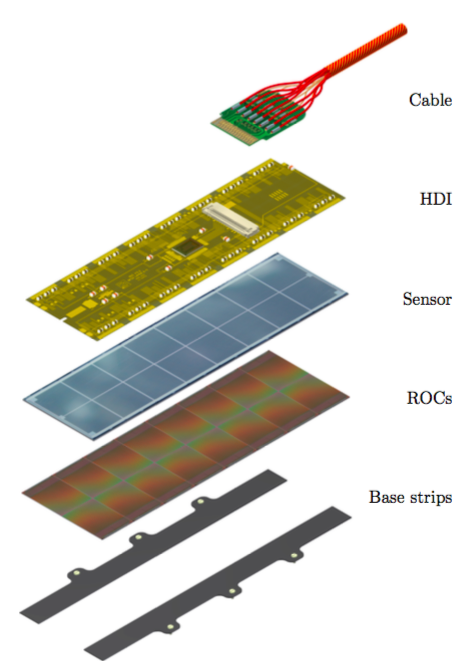
\includegraphics[width=0.3\textwidth]{\chsixteen/phase1module.png}
 \end{center}
 \caption{Exploded view of the the digital pixel module employed for the outer barrel layers of the upgraded BPix detector.}
 \label{fig:Phase1Mod}
\end{figure}

\subsection{The digital ROC}

The ROC for the upgraded detector~\cite{Kastli201388} is not a completely new development but rather an evolution of the well-proven ROC operating in CMS since its commissioning.
It is designed in the same 250\unit{nm} CMOS technology and the well understood core of its double-column architecture is mostly unaltered.
However, to cope with the higher data bandwidth the readout protocol has been changed from a 40\unit{MHz} analog to a 160\unit{MBit/s} digital readout. An ADC digitizes the analog pulse height information in the ROC periphery
The key additional elements are an 8-bit successive approximation current ADC running at 80\unit{MHz} with a programmable range and a PLL which generates the 160 and 80\unit{MHz} for the serial readout links and the ADC respectively, from the 40\unit{MHz} LHC master clock.
To reduce data losses, the number of hit buffer cells in each double column has been increased from 32 to 80 and the time stamp buffers have been increased from 12 to 24.
To limit the increase of the area used by the buffers the layout has been redone completely.
An additional readout buffer stage has been introduced in the ROC periphery to reduce dead time during the column readout: the data is transferred (after being digitized) into the new readout buffer immediately after the trigger arrives and the double columns go live again.
Improved performance of the analog amplifier and the discriminator in the pixel unit cell allow for operation at lower threshold, which is reduced from about 3500 electrons in the current detector to under 2000 electrons after the upgrade. This guarantees higher radiation tolerance and hence, a longer lifetime of the detector.

The chip just described is suitable for the whole upgraded pixel detector except for the innermost barrel layer, where the data rates up to 600\unit{MHz/cm$^2$} are expected, four times higher compared to the second layer.
In order to cope with such extreme conditions the newly developed PROC600~\cite{Starodumov:2227967} readout chip is used in the innermost layer. The new chip features a new 40\unit{MHz} Dynamic Cluster Column Drain mechanism based on dynamic cluster ($2\times2$ pixels) finding in the double column.

\subsection{The TBM and readout}\label{subsec:Phase1TBM}

Differently to the present detector, for the upgrade all barrel modules use at least two data channels in order to improve the bandwidth of the readout.
Because of the limited number of fibres available for this purpose, two channels are always multiplexed into one data stream through a DataKeeper multiplexer and encoder.
For this purpose few modifications have been applied to the TBM.
In particular, it combines the digital 160\unit{Mbit/s} readout from the ROCs from two buses into a 320\unit{Mbit/s} signal to which it then applies 4-to-5 bit encoding. This results in a 400\unit{Mbit/s} data stream.
The readout scheme is adapted to the different barrel layers.
Figure~\ref{fig:Phase1TBMRO} provides an illustration of the readout scheme described in the following.
Layers 3 and 4 employ a dual core TBM, referred to as TBM08, that passes two tokens simultaneously to achieve the parallel readout of two groups of 8 ROCs, called Port 0 (or Channel $\alpha$) and Port 1 (or Channel $\beta$). 
The data are then combined into one data stream as described above, requiring one fibre. Except for the multiplexing step, this is very similar to the method used for the first two layers of the present detector (Fig.~\ref{fig:TBMreadout}).
Layer 2 employs a different TBM, called TBM09, which is the equivalent of two TBM08s (TBM A and TBM B in Fig.~\ref{fig:Phase1TBMRO}), each equipped with its own DataKeeper. This TBM is capable of issuing four tokens simultaneously so that the 16 ROCs are therefore divided into four groups that are readout in parallel. The two DataKeepers then produce one 400\unit{Mbit/s} data stream each and two fibers are required for the readout.
For the innermost layer two identical TBM09 chips per module are employed and identified by two different HUB addresses. In this case eight tokens are passed in parallel on these modules, resulting in four 400\unit{Mbit/s} data streams and hence, four fibers for transmission.

An extensive set of control registers have been built into the TBM, which allow various functions and operating modes of the TBM to be controlled by issuing commands to the TBM through the communication control HUB.
For the TBM09 the commands have to be issued to both TBM08s controlled by one unique HUB.

\begin{figure}[!htb]
 \begin{center}
 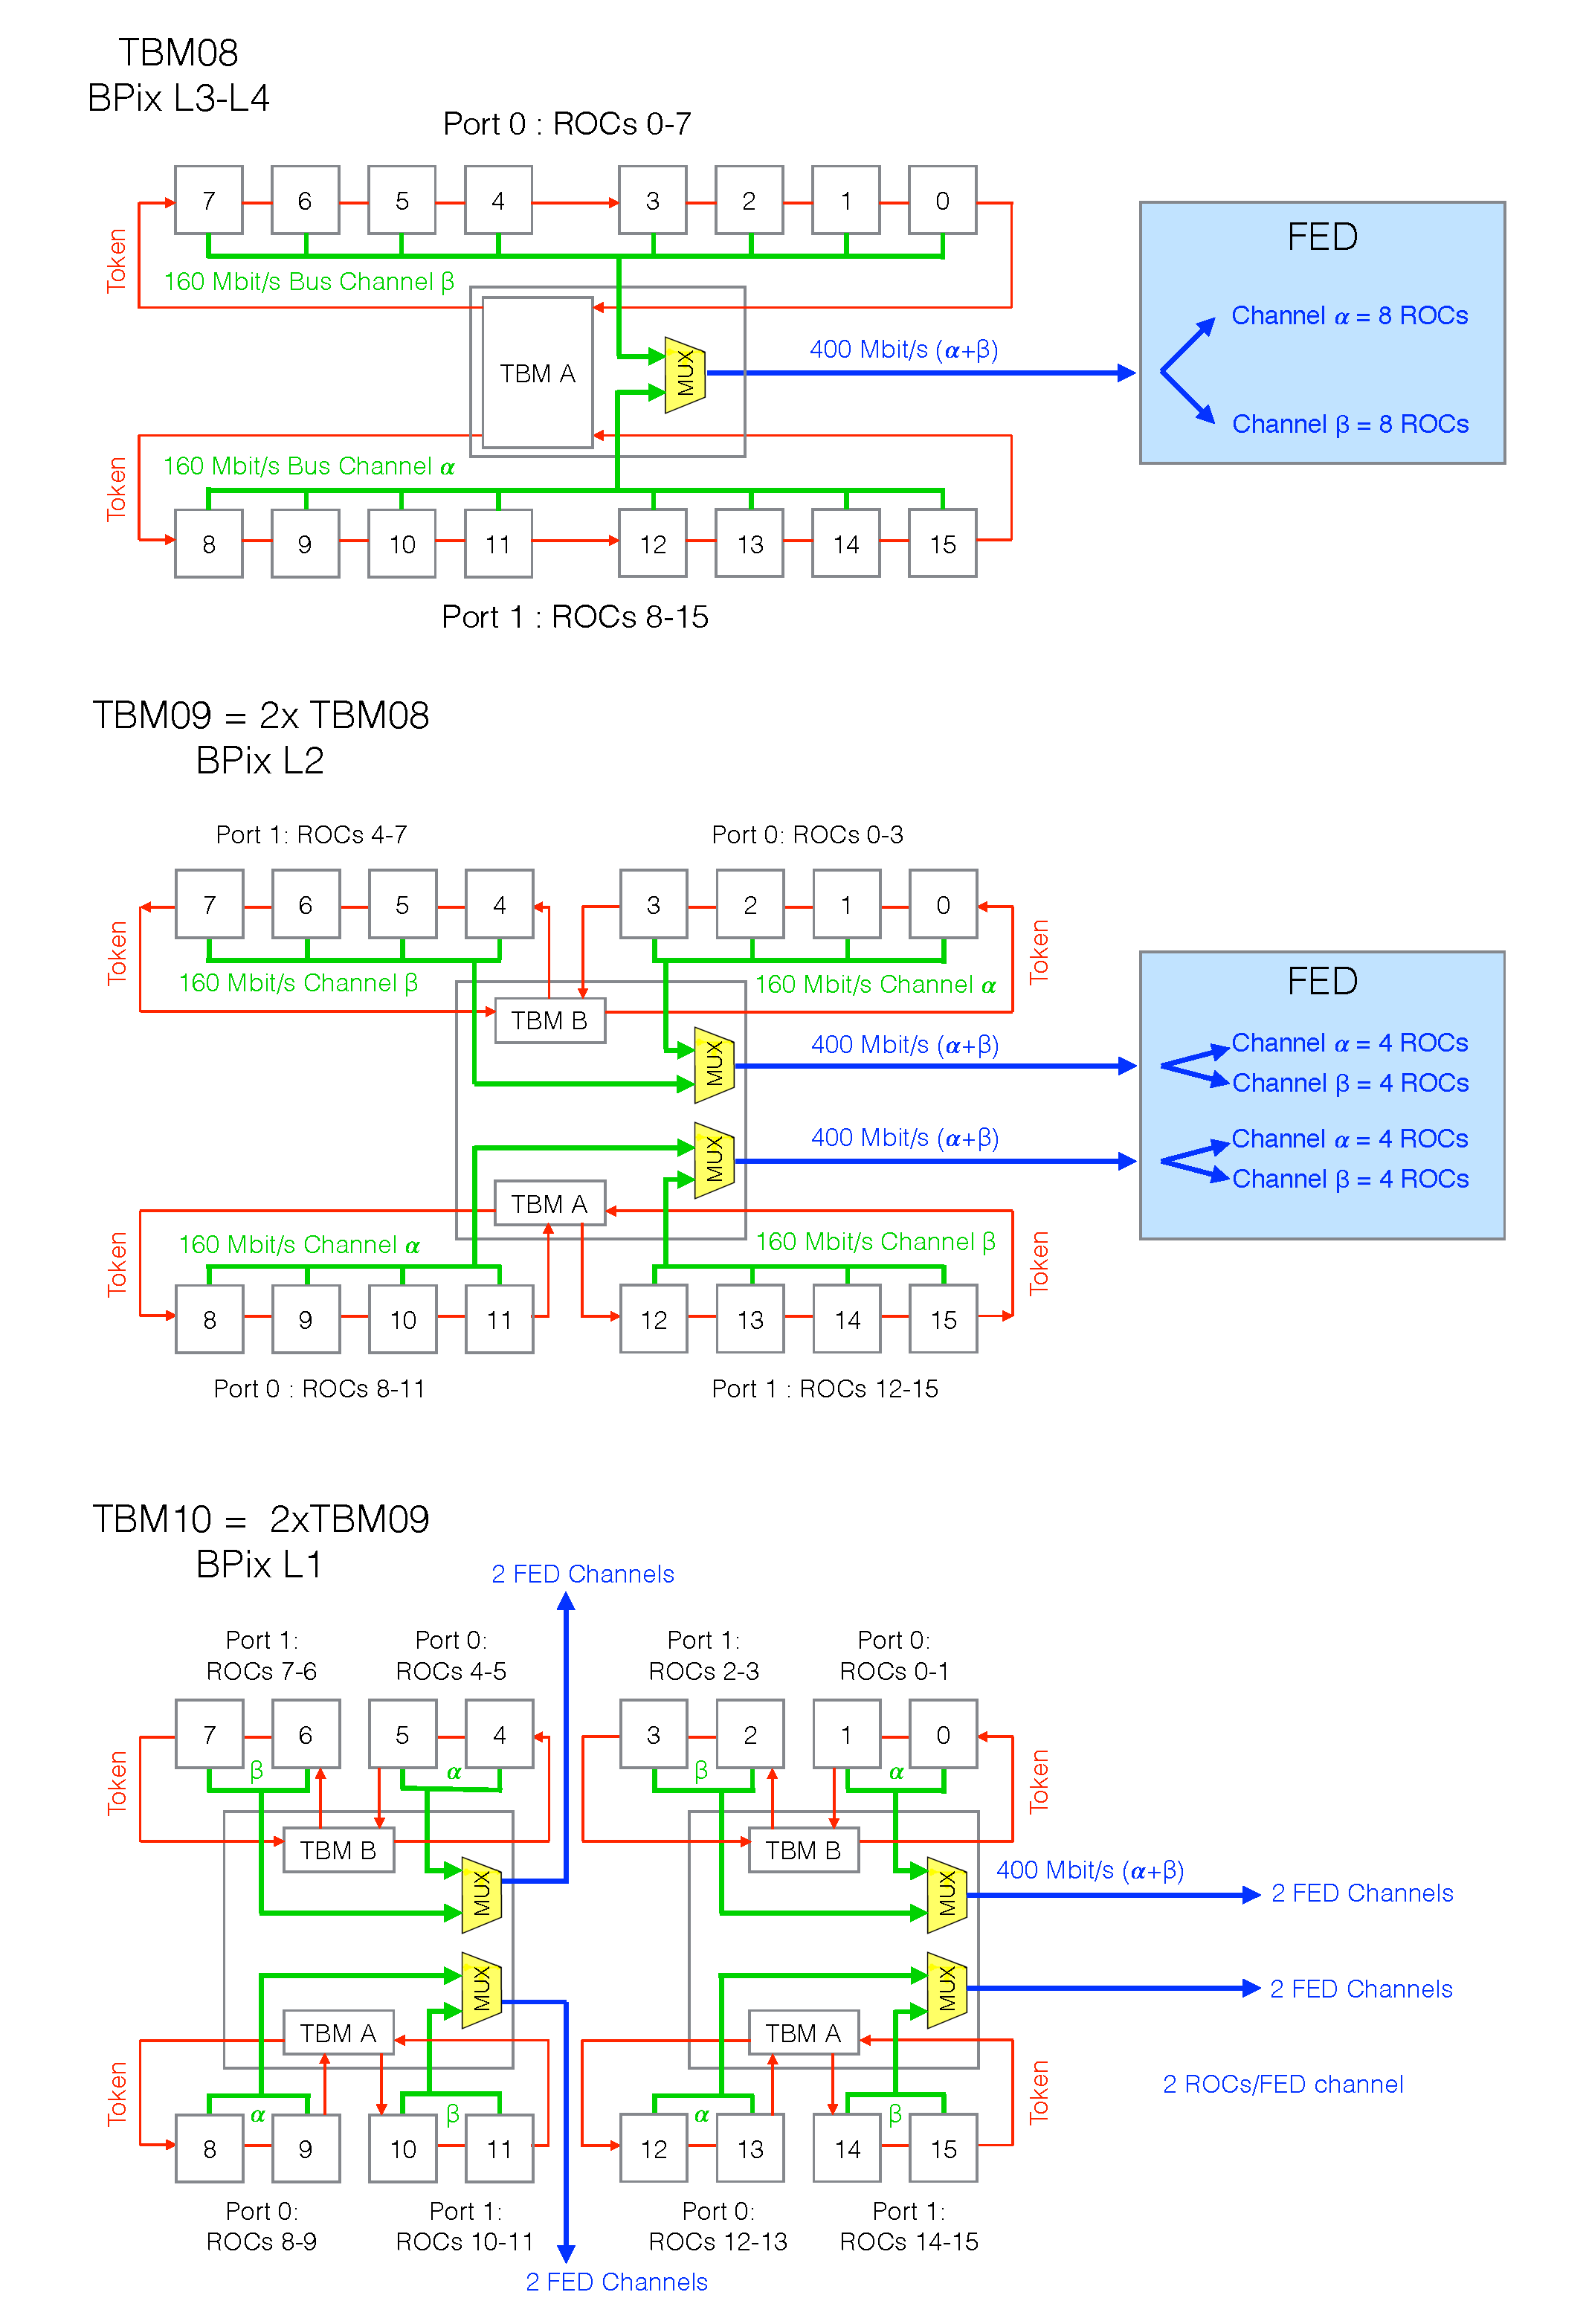
\includegraphics[width=\textwidth]{\chsixteen/AllTBMs.pdf}
 \end{center}
 \caption{Readout scheme of the different TBMs used in the BPix layers.}
 \label{fig:Phase1TBMRO}
\end{figure}

As for the present detector the module output signal is characterized by TBM header and trailer, ROC headers and pixel hit information, which are now encoded in binary data as shown in Fig.~\ref{fig:digTBMRO}.
A TBM readout begins by transmitting a twelve clock cycle (160\unit{MHz}) header sequence.
The next sixteen clock cycles of the header are used to transmit the 8-bit event counter, 2 bits of error information, and a 6-bit stack count value.
Coincident with the next to last clock cycle, the token is transmitted to the ROCs. The TBM now goes into standby mode, waiting for the last ROC in the chain to return the token to the TBM.
At this stage, the TBM transmits a twelve clock cycle trailer sequence. This contains 8 bits of error status, and 8 bits encoding the data contained in the last 8-bit TBM register accessed.
The TBM also contains a timeout on the token returning. It the token fails to return, before the timer expires, the TBM will automatically issue a ROC reset, ending the token pass.
The data contained in the ROCs are deleted, and error bits are returned in the TBM trailer 8 clock cycles later.
The ROC data consist of 12 bits for the header, 16 bits give the pixel hit address and the final 8 bits tell the pulse height.\\

In order to readout the new fully digital pixel system a VME-digital FED has been firstly designed.
It is a hybrid solution with new daughter boards on the existing FED and it has been used at the beginning of the operation with the pilot system and in the test stands.
This solution will be replaced by a $\mu$TCA system with high-speed signal links providing data rates up to 10\unit{Gbits/sec}. 
Since the results presented in this work are based on the VME back-end system, only this is described in the following.

The ADC daughter boards of the analog FED are not needed anymore for digital transmission.
For the purpose of system development, a special add-on board was produced which is mounted on the current VME module for data readout, receives the 400\unit{Mbit/s} digitized data, and passes the data to the VME module in the same format as the current system.
%A plug-in replacement board has been designed holding a new receiver modified to operate at a higher wavelength,
%as well as an FPGA which will be used for synchronization and deserialization of the incoming data in a way that is transparent to the subsequent electronics.
Thanks to this modular approach, the other parts of the FED did not require any hardware modification allowing for a quick start of the tests with the new upgraded pixel system.

As shown in Fig.~\ref{fig:Phase1TBMRO}, the signal from each fiber is split at the FED into two channels whose content is buffered and processed in the FIFOs.
Each channel will then correspond to the data from half of the initial number of ROCs present in one fiber.

\clearpage

\begin{figure}[!htb]
 \begin{center}
 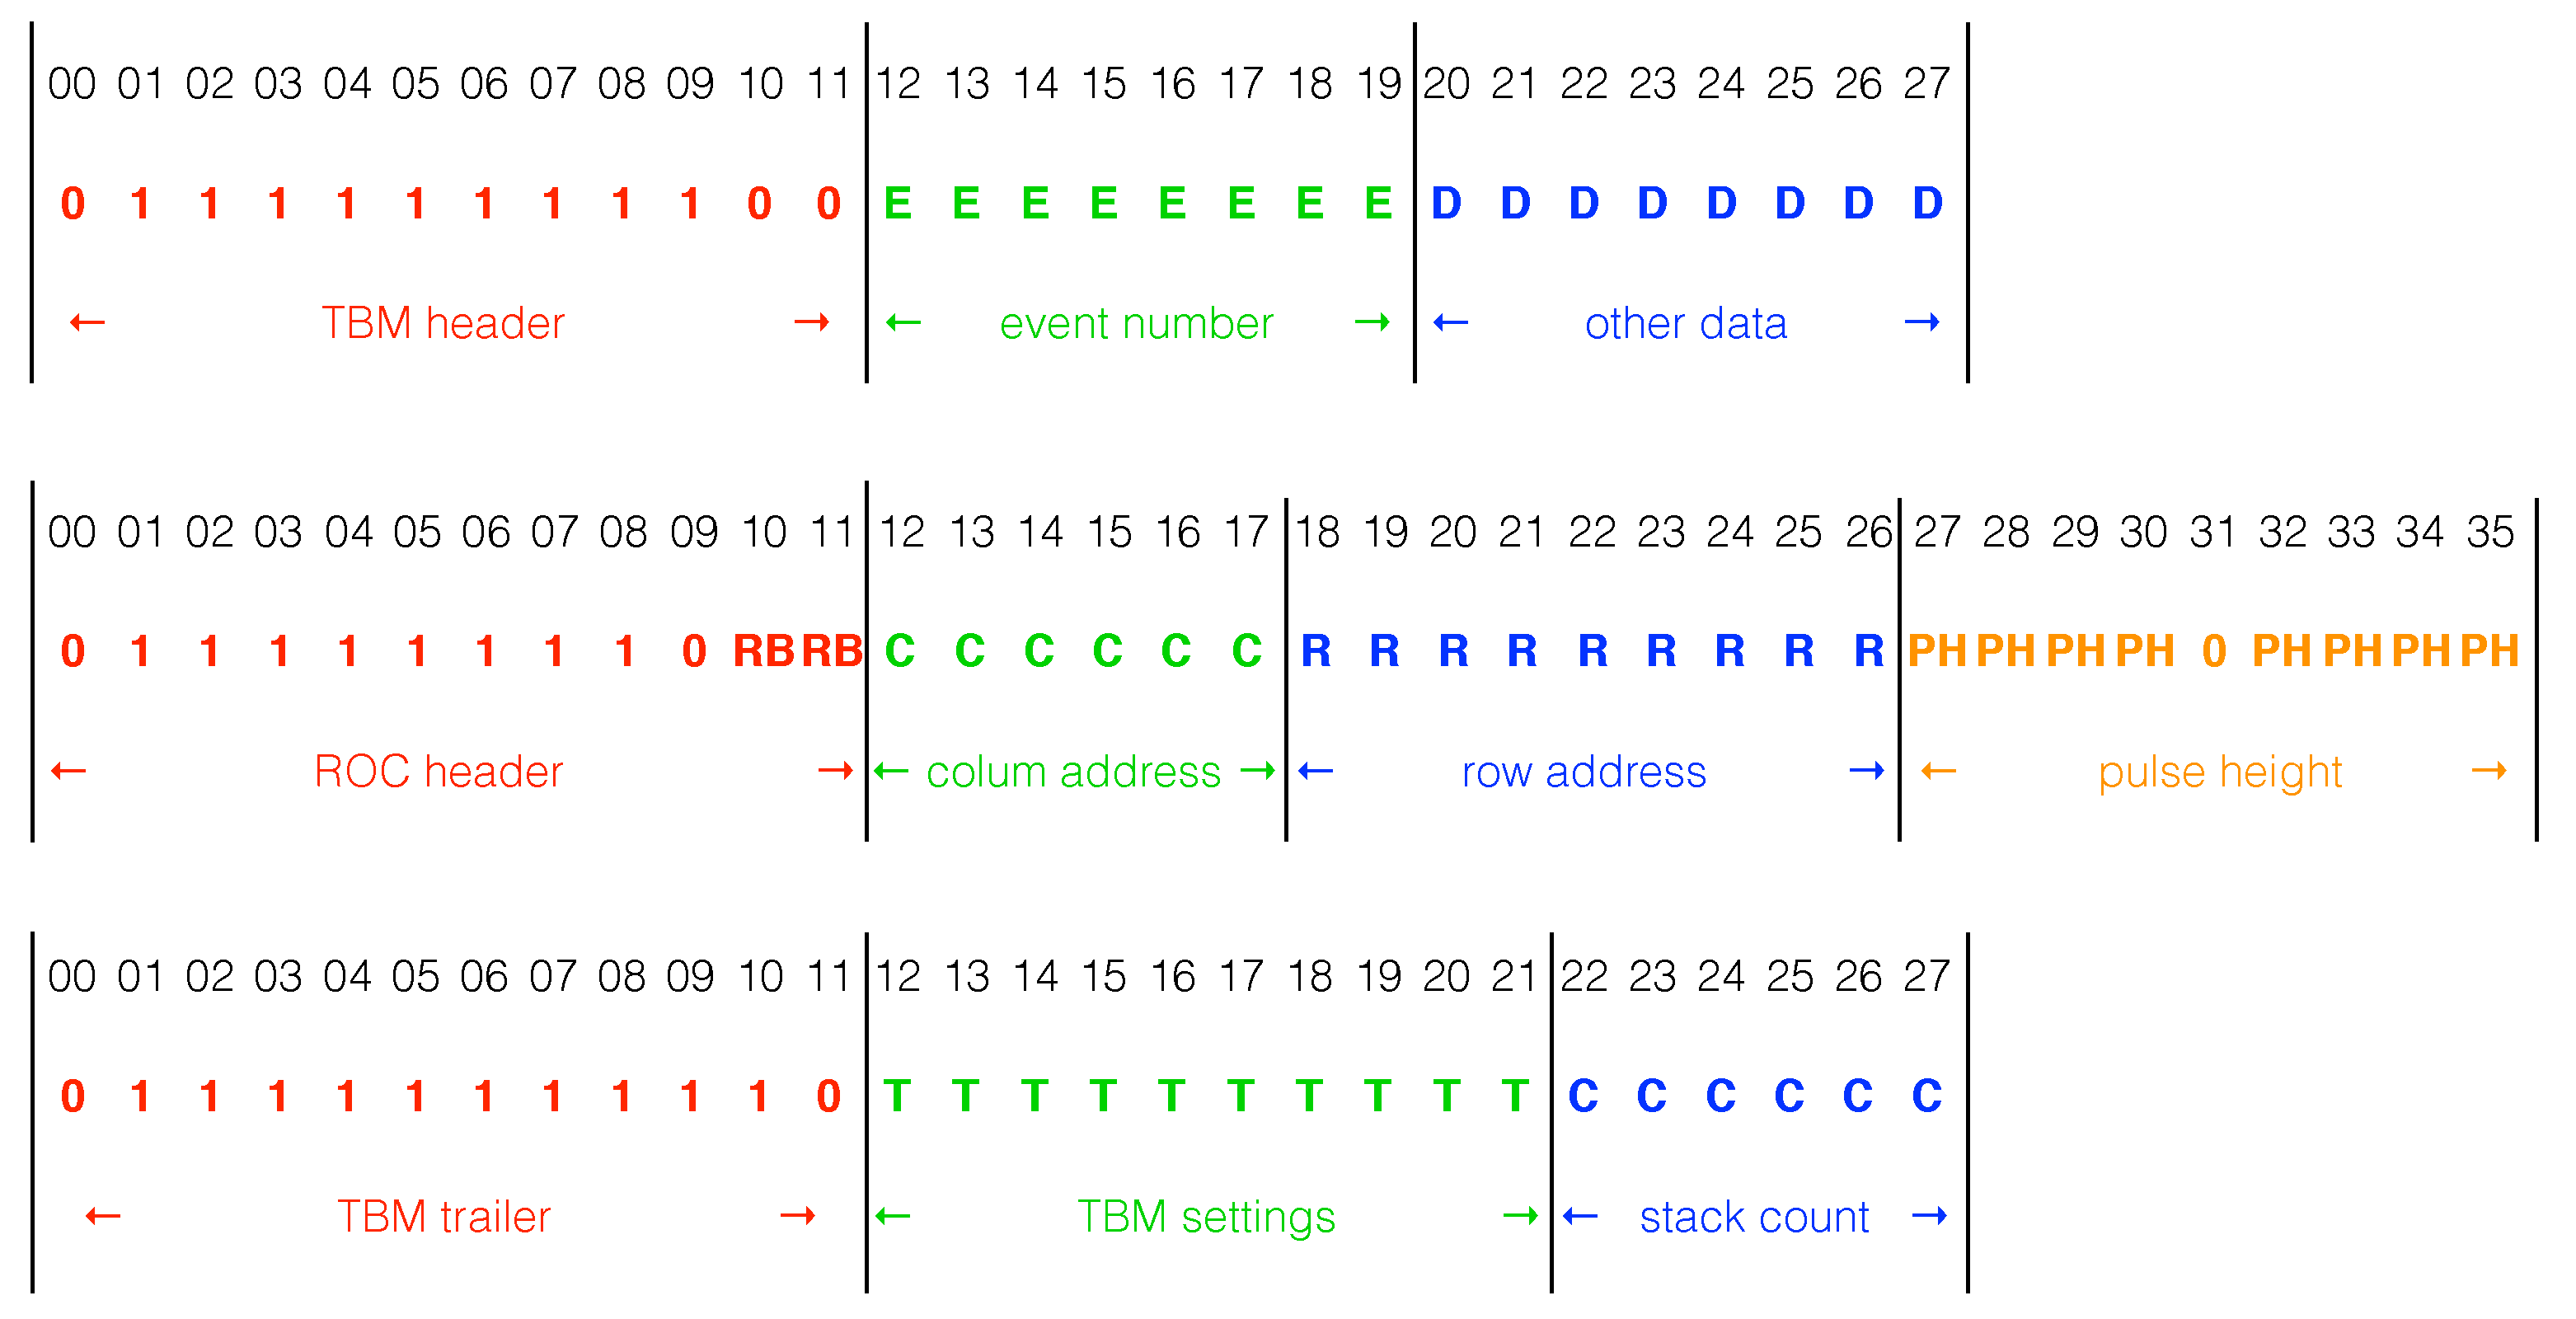
\includegraphics[width=\textwidth]{\chsixteen/digitalTBMreadout.pdf}
 \end{center}
 \caption{Decoding of the TBM output data.}
 \label{fig:digTBMRO}
\end{figure}

%%%%%%%%%%%%%%%%%%%%%%%%%%%%%%
\section{Supply tubes}
%%%%%%%%%%%%%%%%%%%%%%%%%%%%%%

As for the present detector, the power, readout and control circuits as well as the cooling lines are housed by four half-cylinder supply tubes.
The mechanical structure of the service cylinders is made from layers of carbon fiber composites.
Each cylinder is divided in sectors which hold the electronics for one readout group of detector modules.
Figure~\ref{fig:phase1SC} shows the layout of one half cylinder together with some of the new electronic components.
Each sector includes DOHs as well as the auxiliary chips (PLL, Delay25, Gate-Keeper) for the transmission of control, clock and trigger signals.
So-called pixel opto-hybrids (POHs)~\cite{1748-0221-7-01-C01113} are used for the transmission of the module readout data as a replacement of the AOHs used for the present detector.
The change from analog to digital module readout in the upgrade system also requires the adoption of new optical links.
POHs are built from four transmitter optical subassemblies (TOSA), linear laser-driver and level-translator chips and have been designed specifically for their use in the pixel upgrade system.
All other components used in the control and readout chain are identical to the ones used in the current system. CCU chips are used for slow control, monitoring and timing distribution.
Furthermore, pairs of DC-DC converters are mounted on the service cylinders.
Each sector consists of a stack of boards, DC-DC converters, optical links and cooling loops, resulting in tight space constraints and a non-trivial assembly procedure.
%The DC- DC converters operate at an input voltage of 10 V with an output voltage of 2.4 V and 3.3 V for the analog and the digital voltage supply of the modules, respectively, with an efficiency of about 80%. The choice of the converter output voltage takes into account the voltage drop across the service cylinder and guarantees a minimum supply voltage of 1.6 V and 2.4 V for the analog and digital nodes of the modules, respectively. Each converter can provide up to 3 A of current and a total of 1184 DC-DC converters is used for the full detector system. The service cylinders of the BPIX and the FPIX are shown schematically in Figure 3.  

The complete supply tube system has been integrated and tested sector by sector at the University of Zurich.\FIXME{add nice picture from UZH}

\begin{figure}[!htb]
 \begin{center}
 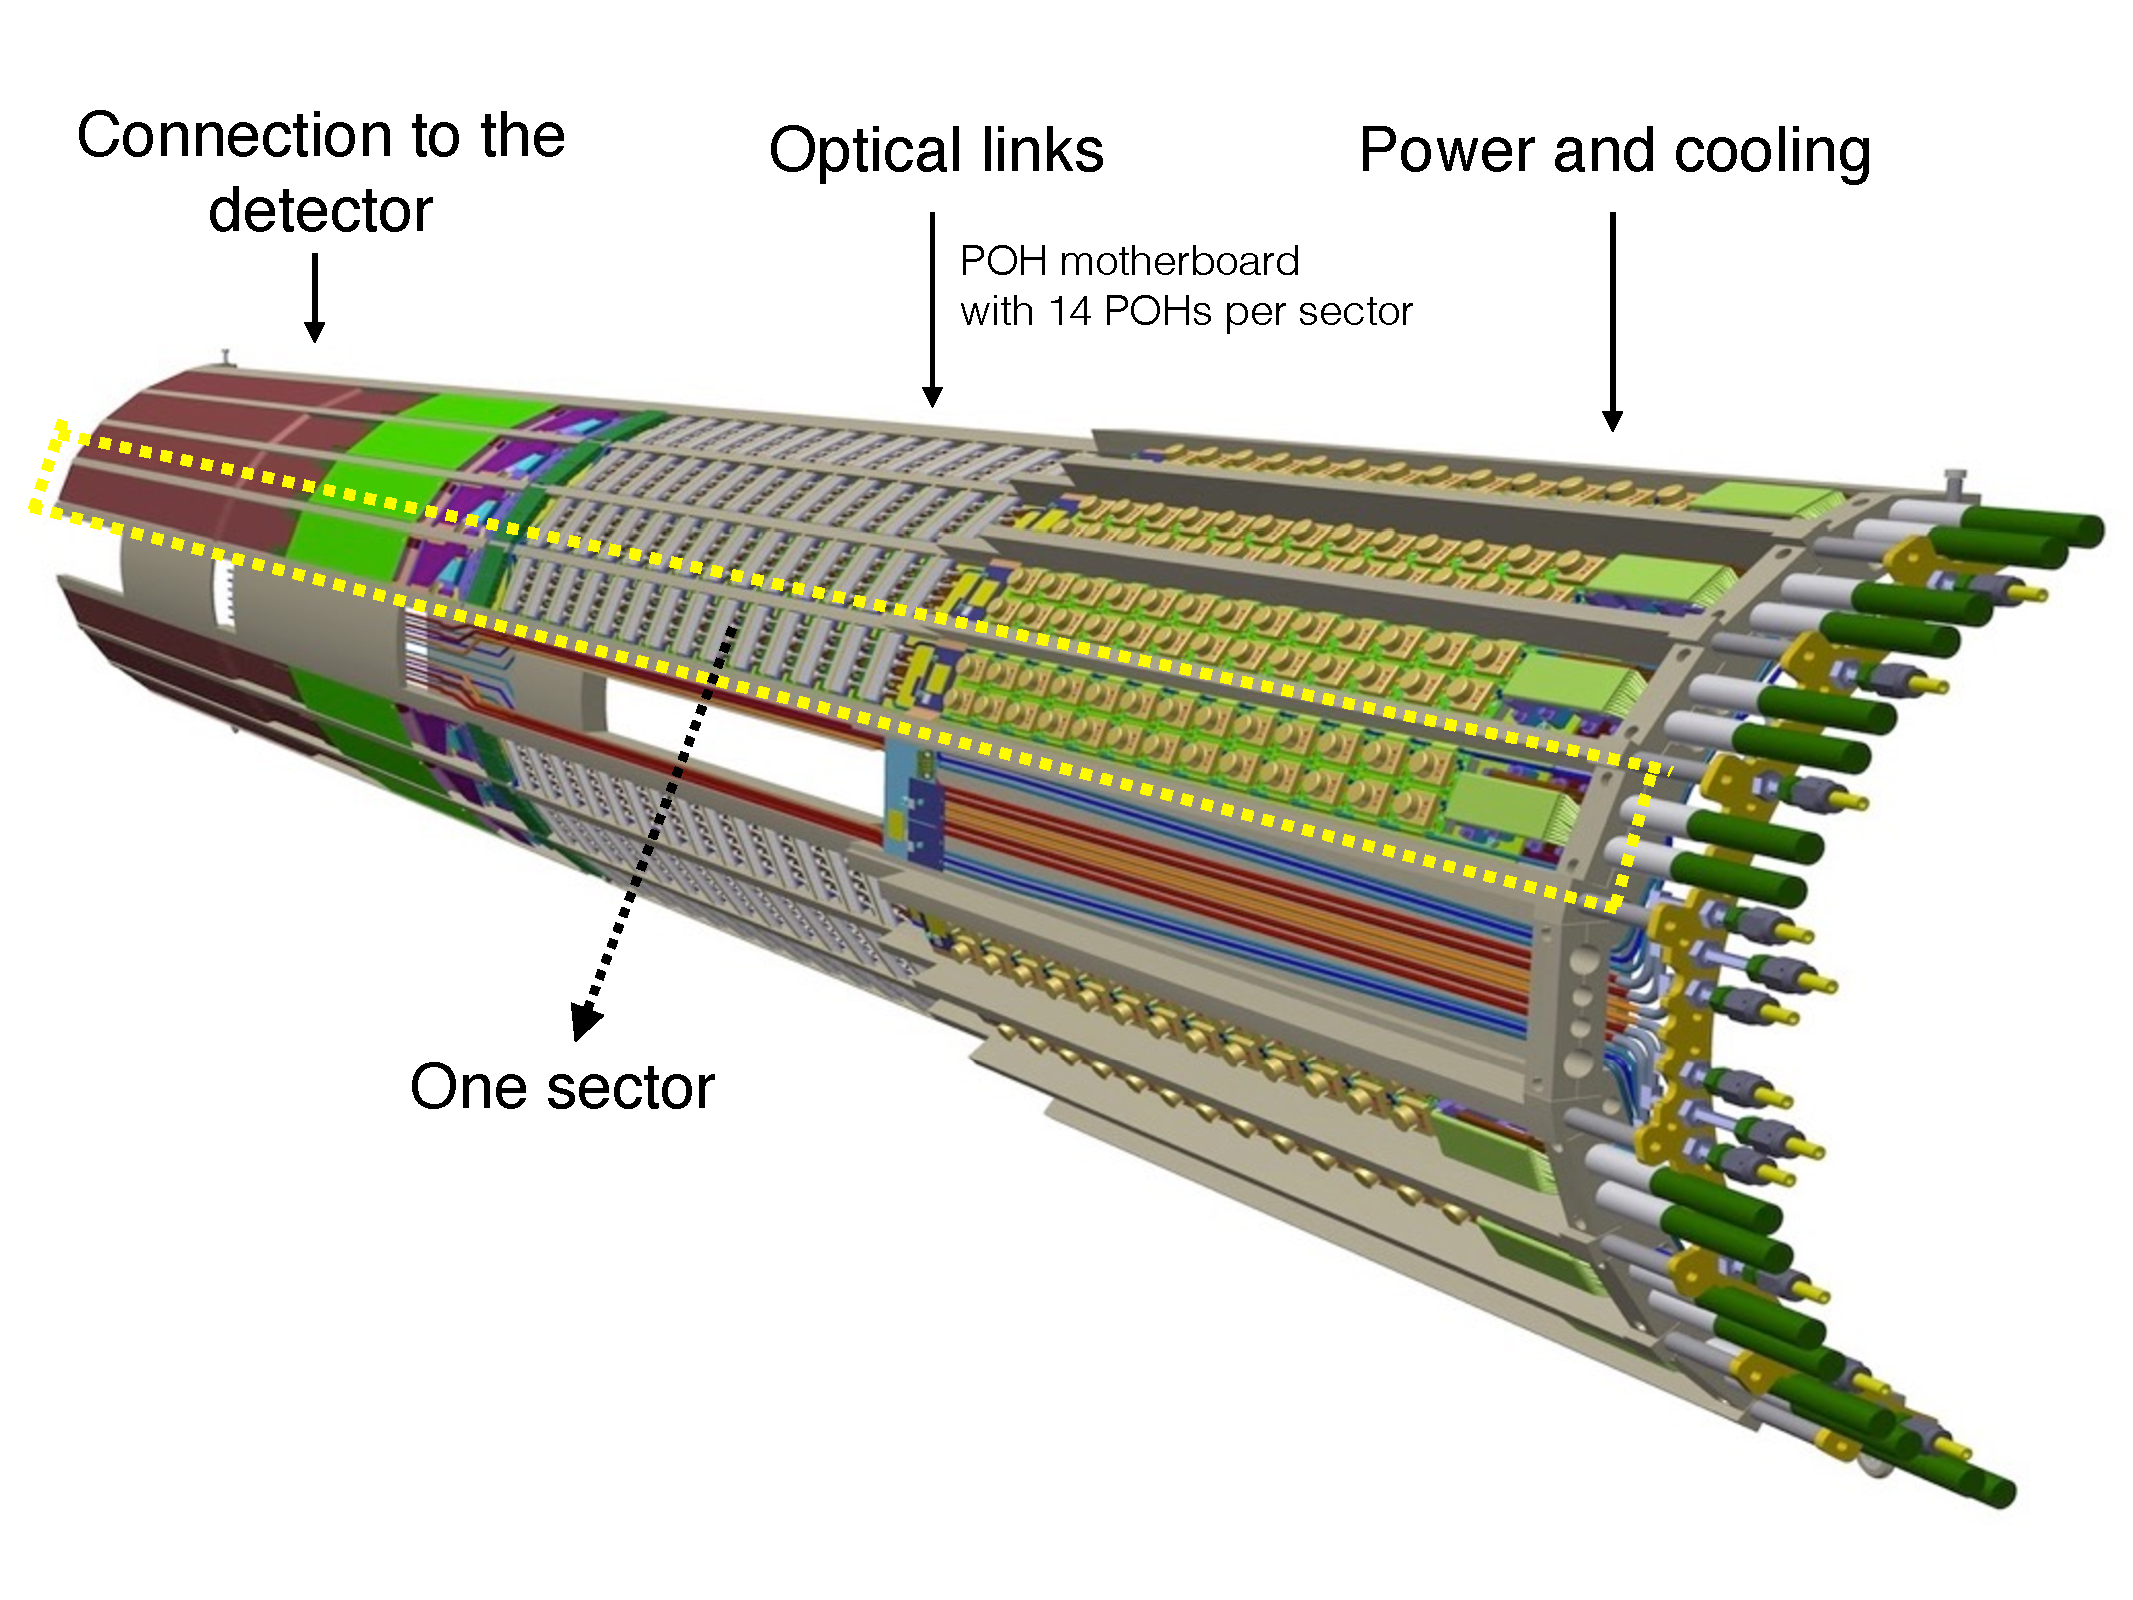
\includegraphics[width=0.7\textwidth]{\chsixteen/SC-layout.pdf}
 %\subfigure[]{\label{fig:phase1SC_b}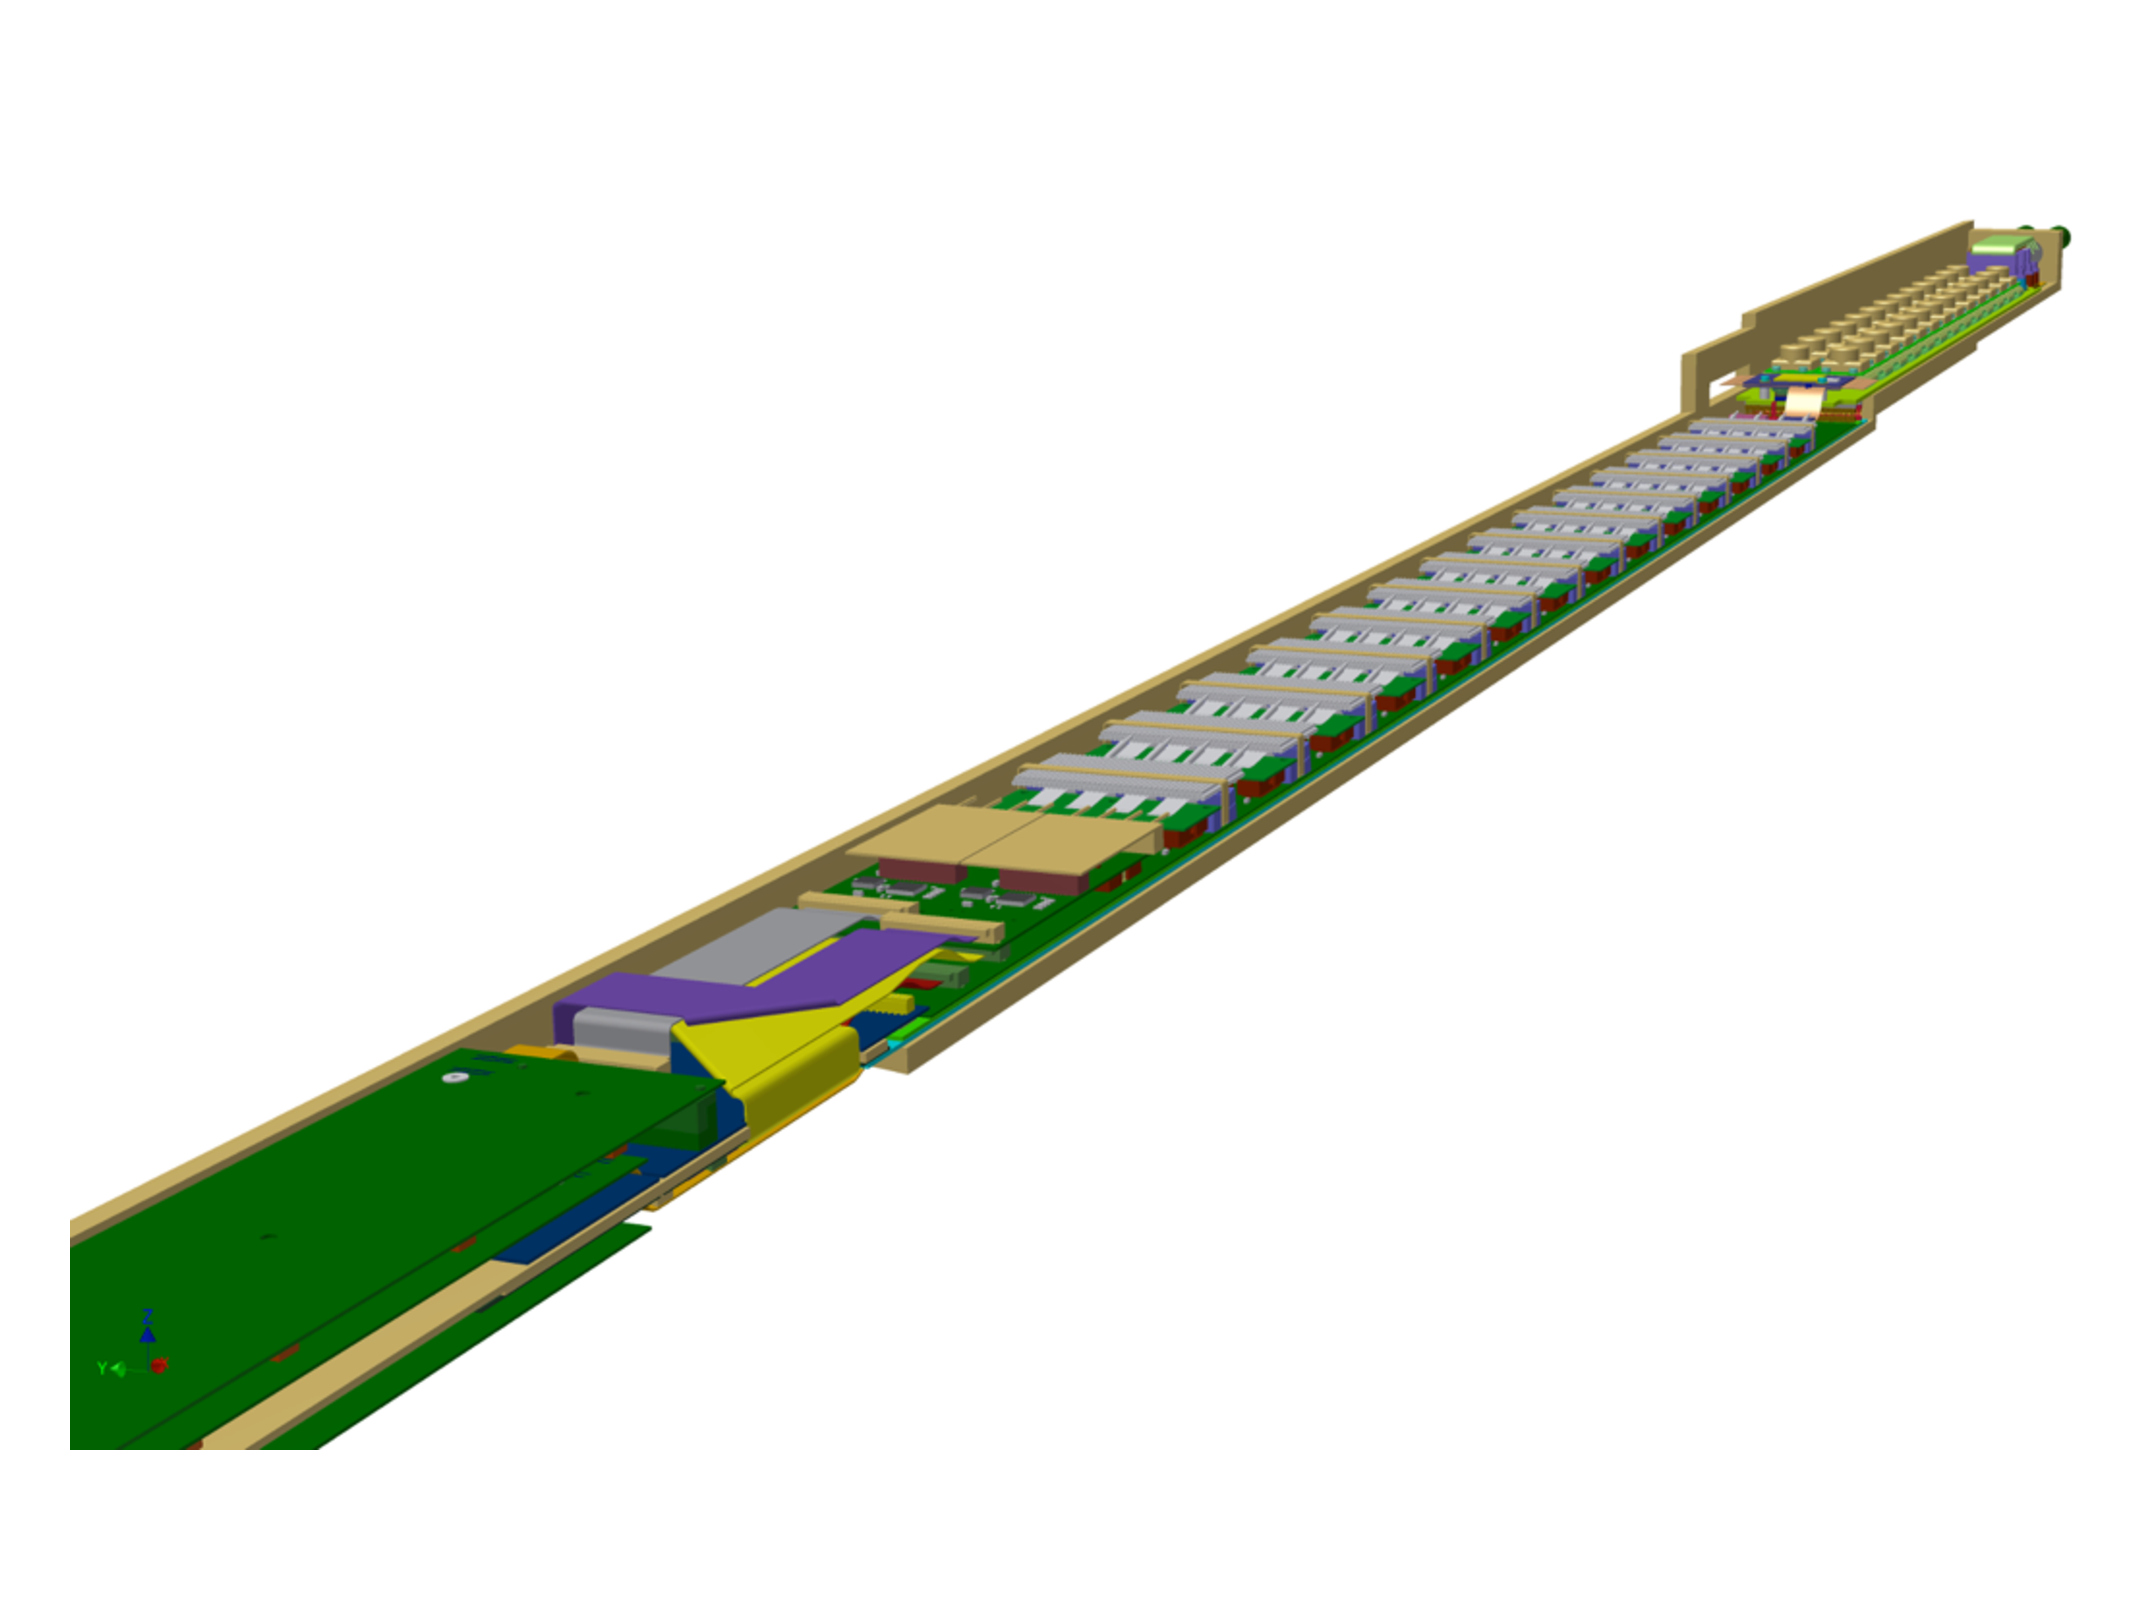
\includegraphics[width=0.4\textwidth]{\chsixteen/SC-stack.pdf}}
 \end{center}
 \caption{Layout of one of the four supply tube half cylinders for BPix equipped with the new electronic components. Each half cylinder is divided into 8 sectors.}
 \label{fig:phase1SC}
\end{figure}

%%%%%%%%%%%%%%%%%%%%%%%%%%%%%%
\section{The test stand}
%%%%%%%%%%%%%%%%%%%%%%%%%%%%%%

In order to test the performance of the complete upgrade pixel system and gain experience in its operations, a test stand for BPix has been set up at the University of Zurich in 2013.
The setup includes a slice of the full CMS pixel DAQ system together with prototypes of all components of the upgrade power system, control and readout chain as well as a number of detector modules.
The system test was operated until November 2016 when the integration of the supply tubes started.
Its main goals included:
\begin{itemize}
\item test all components of the detector system prior to full production;
\item test all final components before and after integration on the supply tubes;
\item establish test and calibration procedures for the assembly and commissioning (Section~\ref{sec:Phase1Calib});
\item exercise the transition from the VME- to the $\mu$TCA-based DAQ system.
\end{itemize}

Figure~\ref{fig:TestStandUZH} shows a picture of the test stand,
which consists of several sensor modules, electronics for their operation, a CAEN power supply and a VME back-end system to control and readout the modules.
The test stand is also equipped with a linux PC connected to the VME and used to run and control the system through the installed XDAQ applications.
%say that we do have computers to run and control the system
%say that the supply tubes testing is done with BPixTools. contributed to find and apply changes to this software to make it work with the new configurations.
%say that afterwards I installed POS and that I had to make foundamental changes to make it work with the test system.

\begin{figure}[!htb]
 \begin{center}
 \includegraphics[width=\textwidth]{\chsixteen/UZHteststand.pdf}
 \end{center}
 \caption{Test stand setup at UZH including all components of one BPix sector together with a few pixel modules. The CAEN power supply and the VME back-end system are also indicated.}
 \label{fig:TestStandUZH}
\end{figure} 

Most of the tests that have been conducted with this system make use of a standalone software based on the socket technology provided by the \textsc{Python} framework.
that allow for a direct communication with the hardware. 
%Through the Python socket interface the user can send messages to the control processes and receive the answers.
These tools have been firstly developed for the testing of the present pixel detector prior to assembly\cite{Caminada:2010gsa} and necessitated many fundamental changes to be able to operate with the upgraded system.
I implemented part of this transition and I was able to perform the first tests with the POHs.
In the example shown in Fig.~\ref{fig:TestPOH} the POH laser bias setting is varied from 0 to 40 and for each value the ADC counts (or optical power) at the analog VME FED are checked.
This scan is performed for different values of POH laser gain setting.
The optical power sharply increases until the saturation of the receiver at the FED is reached.
This test firstly ensured the slow I$^2$C communication with the auxiliary electronic components of the system.
Other tests have been performed after pixel modules have been added to the system and  aimed at establishing the functionality of the fast I$^2$C communication to/from the TBM.
This was checked by verifying for instance the presence of the TBM signal at the corresponding POH output through an optical probe plugged into the oscilloscope.
If the fast I$^2$C communication through the digital circuit is functional, the TBM sends the 400\unit{Mbit/s} data stream upon the arrival of a trigger as shown in Fig.~\ref{fig:TestTBM}.

\begin{figure}[!htb]
 \begin{center}
  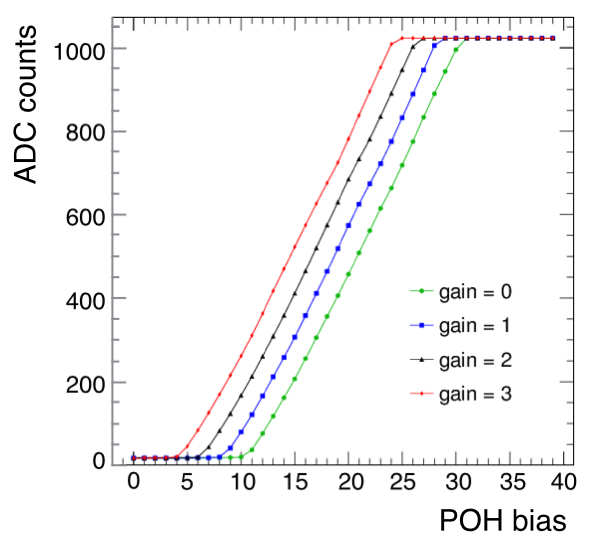
\includegraphics[width=0.45\textwidth]{\chsixteen/POH-bias-scan.png}
 \end{center}
 \caption{Typical result of the scan of a POH laser bias and gain. For each value of the laser settings, the optical power is readout at the VME-analog FED.}
 \label{fig:TestPOH}
\end{figure} 

\begin{figure}[!htb]
 \begin{center}
  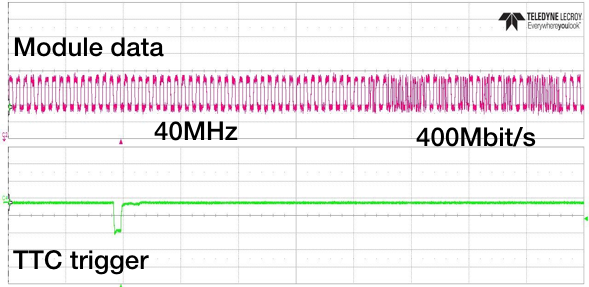
\includegraphics[width=0.7\textwidth]{\chsixteen/TBMsignalOscilloscope.png}
 \end{center}
 \caption{Module output signal initialized by a trigger sent by the TTC. The signal is acquired at the oscilloscope with an optical probe connected to the POH laser output. The 400\unit{Mbit/s} signal contains TBM trailer and header, and the header from 8 ROCs.}
 \label{fig:TestTBM}
\end{figure} 

These kinds of test are not suitable when dealing with a large number of channels. For detector assembly and commissioning the full functionality of each module has to be checked and calibrations have to be performed over the whole detector. In order to achieve this in a reasonable amount of time the full pixel online software (Section~\ref{sec:BPix_POS}) has to be used and upgraded to be able to operate with the new system.
Many fundamental changes to the software have been firstly applied for the pilot system as well as for operations with the FPix test stand at CERN.
These changes mainly concerned the \texttt{FEDInterface} class where the new features of the digital VME-FED had to be implemented.
In order to test and debug the new developments I installed POS and applied the modifications required to run it with the system test at UZH.
After establishing the basic functionalities, I developed new calibrations for the upgraded detector as described in the next section.
%This work has been crucial to understand, implement and test new features for the software needed to be able to operate specifically with the BPix detector.
This work represents the first attempt to operate the upgraded BPix system with POS and hence, has been crucial to understand, implement and test new BPix specific developments.

In mid-2016 a separate table has been setup in the same laboratory to operate the upgraded electronics with the $\mu$TCA DAQ system as this became available only at a later time.
A new $\mu$TCA-based version of POS was developed in the meantime by the FPix group and the second test stand has been very useful to gain expertise with the new developments.
Several of the new features for the upgraded system that I included in the VME-POS have been easily exported to the $\mu$TCA-POS.
The transition has been straightforward since I developed the new code such that it is transparent with respect to the parts of the software handling the $\mu$TCA or VME communication.

%%%%%%%%%%%%%%%%%%%%%%%%%%%%%% 
\section{Testing and calibration}\label{sec:Phase1Calib}
%%%%%%%%%%%%%%%%%%%%%%%%%%%%%%

Since the upgraded system features a new digital readout some of the steps of the calibration procedures for the current detector become obsolete while new kind of tests are needed.
In particular, the adjustment of the FED receiver offset, of the UB and address levels are dropped for obvious reasons.
Furthermore, since the digital FED is not able to register the optical power, it is not possible to perform a laser bias scan (Fig.~\ref{fig:AOHBias}).
In this section a calibration procedure for the Phase 1 detector is described with main focus on the new developments.
This procedure is suitable for testing each sector of the detector after assembly at PSI as well as for the commissioning of the whole detector at CERN.
It is implemented in several steps, each aimed at testing one particular functionality. 
Each step produces new detector settings, such as POH bias and gain or TBM and ROCs DACs, after a dedicated scan of a set of parameters.
The procedure has been fully tested with the table top system at UZH and few pixel modules and results will be presented and discussed in the following.
Only modules equipped with TBM08 and TBM09 have been used for these tests,
since the TBM10 was not available at the time of this work.
Additionally, since the TBM10 features slightly different readout and programming mechanisms, further modifications to the software were required.
Further improvements to this preliminary version of the procedure have been implemented later on by the BPix group in order to have a finalized version for detector commissioning
that also include specific developments to operate with the TBM10.

\subsection{Delay adjustments}\label{subsec:TBMPLLROCDelays}

The synchronization between the 160\unit{Mbit/s} ROC data and the 400\unit{Mbit/s} final output data stream has to be adjusted in order to be able to correctly readout the module output signal.
%The data alignment can be adjusted by programming several TBM internal registers which control
%\begin{itemize}
%\item the phases of the 160\unit{MHz} and 400\unit{MHz} PLLs integrated in the TBM: they can be changed in the range 0--7\unit{ns} in steps of 1\unit{ns};
%\item the delay in the ROC data signals in the range 0--7\unit{ns} in steps of 1\unit{ns}; %this change can be applied to each of the two readout groups of ROCs of Fig.~\ref{fig:Phase1TBMRO}, called Port0 and Port1;
%\item the delay in the TBM header/trailer by one 160\unit{MHz} clock cycle (6.25\unit{ns});
%\item the delay in the token return by 6.25\unit{ns}.
%\end{itemize}
The data alignment can be adjusted by programming two 8-bit registers internal to the TBM.
The first register controls the phases of the 160\unit{MHz} and 400\unit{MHz} PLLs integrated in the TBM.
For the TBM09 only one of the two cores (TBM A and TBM B in Fig.~\ref{fig:Phase1TBMRO}) has to be programmed since the PLLs are common to both.
The second register controls the delay in the data stream of the two readout groups of ROCs (Port 0 and Port 1 in Fig.~\ref{fig:Phase1TBMRO}) and for TBM09 it has to be programmed for each core.
These 4 parameters can be varied in the range 0--7\unit{ns} in steps of 1\unit{ns} so that 3 bits are sufficient for each of them.

After a calibration of the Delay25 chip that ensures communication between the pxFEC and the modules (Fig.~\ref{fig:Delay25}), the first step is to perform a scan of the TBM PLLs' phases.
For each set of values the digital data are readout at the FED and it is checked that the TBM had sent header and trailer. This is done for a large number of triggers and for each FED channel corresponding to the same module (Fig.~\ref{fig:Phase1TBMRO}).
The TBM header and trailer are only available in the FIFO1 which can be accessed only if the normal data flow to the other FIFOs is interrupted. This is achieved by programming a FED register.
An example of such scan for one module is shown in Fig.~\ref{fig:TBMROCdelays_a} where the efficiency for TBM header and trailer to be recorded is measured as a function of the two phases.
The efficiency is averaged over all the FED channels.
At the end of the test new settings for the TBM are produced, corresponding to a pair of phase values with 100\% efficiency. Since there might be more than one bin corresponding to 100\% efficiency only the first one is chosen. However, this algorithm can be improved by picking a bin from a region that presents small variations. If no 100\% efficiency bins are found, the bin corresponding to the maximum is picked and a error flag is saved in the output file. The histogram with the resulting scan is also saved for each module.
%The presence of bins corresponding to 100\% efficiency indicates that clock, trigger and programming signals are correctly arriving at the pixel modules verifying the functionality of the related lines and electronic components. 
This test ensures that the TBM settings are correct to be able to readout the signal. It is also very useful to have a feedback on the status of the detector, for instance after installation, similarly to the FED baseline calibration for the present detector (Fig.~\ref{fig:FEDBaseline}). In fact, it is verified that clock, trigger and programming signals are correctly arriving at the pixel modules and that the TBM can programmed.
In addition, low efficiency might indicate poor optical connections and the problem can be immediately solved by cleaning the fibers.
Issues in the mapping between modules and FED channels, as well as possible broken channels, can also be identified at this stage.\\

The second step consists of scanning the ROC delays and for each set of values it is checked that each ROC had sent the header.
As for the scan of the scan of the TBM PLLs' phases, this is done for a large number of trigger and the efficiency is measured for each ROC.
For the TBM09 the same value is programmed for the two cores.
A histogram is produced with the efficiency averaged over all ROCs and FED channels for each pair of delay values, as shown in Fig.~\ref{fig:TBMROCdelays_b}.
New settings for the TBM are also produced, corresponding to the delay values giving 16 ROC headers recorded at the FED.
The choice of the best settings follows the same strategy described above for the TBM PLLs' phases.
This test ensures that the TBM settings are correct to be able to readout the signal and it also verifies the functionality of the token passage.
%Furthermore, during detector assembly and testing, it is a useful test to check that the number of ROCs per FED channel indicated in the mapping is correct.

\begin{figure}[!htb]
 \begin{center}
  \subfigure[]{\label{fig:TBMROCdelays_a}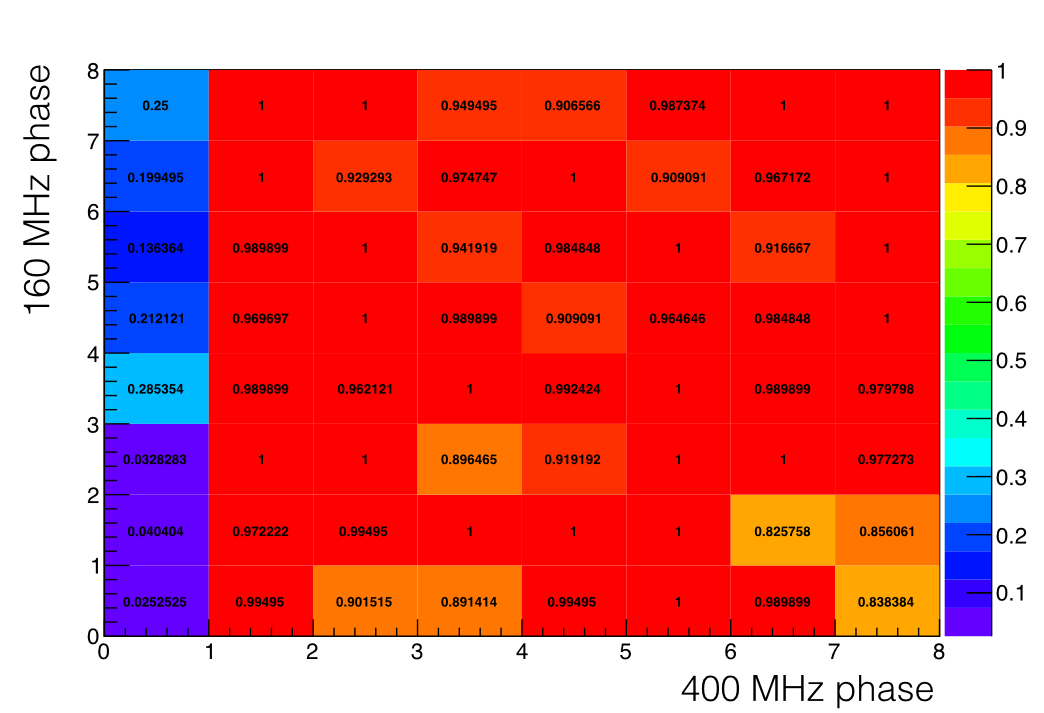
\includegraphics[width=0.45\textwidth]{\chsixteen/TBMPLLDelayCalib.png}}
  \subfigure[]{\label{fig:TBMROCdelays_b}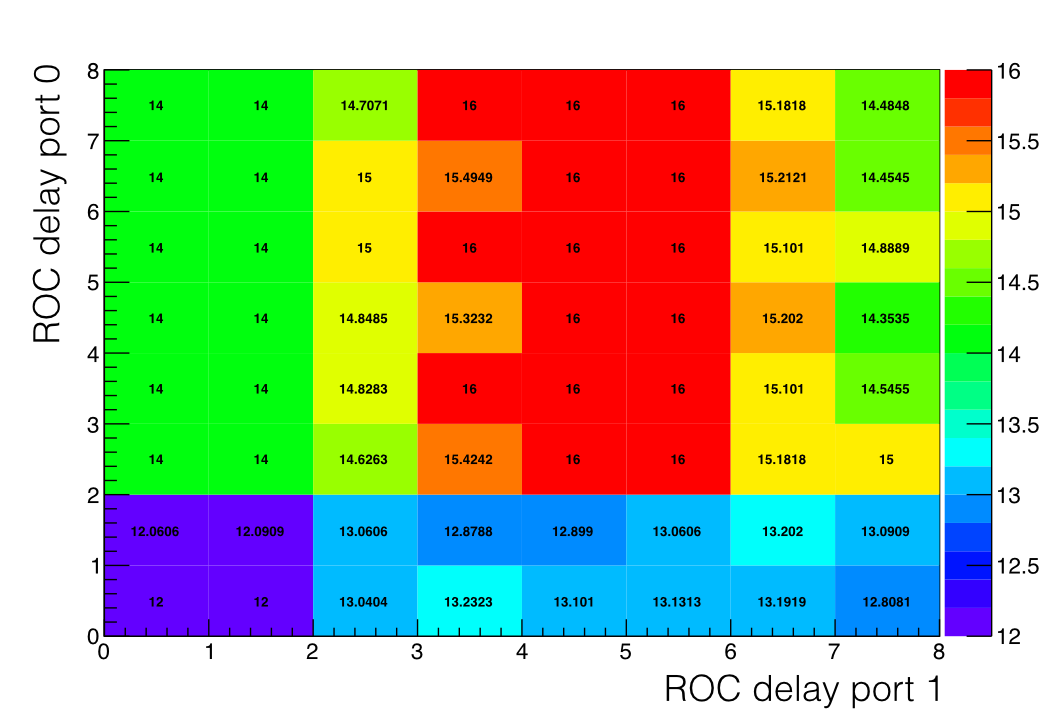
\includegraphics[width=0.45\textwidth]{\chsixteen/ROCDelayCalib.png}}
 \end{center}
 \caption{(a) Example of scan of the 2 TBM PLLs' phases for one module. For each pair of values the module signal is readout several times at the digital FED and the presence of TBM header and trailer is verified.
 An efficiency is obtained by dividing by the number of times the signal has been readout.
 (b) Example of scan of the delay in the ROC data for the two ROC readout groups. For each pair of values the presence of each ROC header in the readout data is verified. The average number of ROCs that sent the header is obtained by dividing by the number of times the signal has been readout.}
 \label{fig:TBMROCdelays}
\end{figure} 

\subsection{POH bias and gain}

The tests described in the previous section assume that the POH laser settings are good enough to allow for a correct readout of the signal.
In fact, a too low laser bias and gain result in a small difference between the 0 and 1 levels of the digital signal and consequently to a large error bit rate.
It has been found with the test stand that a bias of 40 and a gain of 3 are sufficient to be able to correctly readout the signal so that the tests of the previous section can be safely run with such values.
However, once the functionality of the TBM has been verified a scan of the POH setting should be run to obtain a finer adjustment aimed at minimizing the power consumption.
As already mentioned, measuring the optical power as a function of the laser settings is not possible with the digital FED
while an approximate indication of the error bit rate can be obtained by measuring the known TBM signal.
A scan of the POH bias and gain is performed and for each value it is checked that the TBM had sent header and trailer. An example of such scan is shown in Fig.~\ref{fig:POHBiasCalib}.
At the end of this calibration new settings are produced corresponding to a safe area (5 units above the beginning of the plateau).

\begin{figure}[!htb]
 \begin{center}
  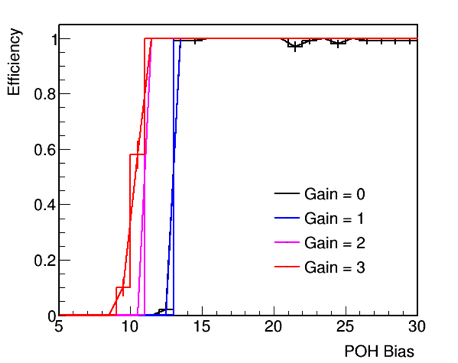
\includegraphics[width=0.45\textwidth]{\chsixteen/POHBiasCalib.png}
 \end{center}
 \caption{Example of scan of a POH laser bias and gain. For each value of the laser settings the module signal is readout several times at the digital FED and the presence of TBM header and trailer is verified.}
 \label{fig:POHBiasCalib}
\end{figure} 

\subsection{Read back test}

As discussed in Section~\ref{subsec:Phase1TBM}, the ROC header is followed by 3 bits where the first one is always a 0 and the other 2 contains the so called read back data.
These data contain different information depending on the value programmed in the ROC read back register. For instance, for a value equal to 12 the ROC analog current is returned.
It has been found after several tests that not all delay settings allow for a correct readout of the information contained in the ROC data stream.
Hence, another scan of the TBM PLLs' phases and ROC delays is performed and for each value the information in the read back data is verified, as explained in the following.

The read back word is encoded in 16 bits (Table~\ref{tab:ReadBack}) which cannot be sent at once given the limited size of the ROC data stream.
As mentioned above there are 2 bits available for the read back data and sent every time the readout is initialized by a trigger.
Of these two, only one belongs to the actual information, so that 16 triggers have to be sent before the entire word can be decoded.
The second bit is used to indicate the start of the word.
Of the 16 bits collected, the first 8-bits are used for the required information (for instance the analog current),
4 bits contain the value written to the read back register (for instance 12 for the analog current),
and the last 4 bits encode the ROC I$^2$C address (from 0 to 15).

%The only a priori known information contained in this word is the ROC I$^2$C address (from 0 to 16) that can be verified.
In order to ensure that the TBM settings chosen by the previous algorithms allow for a correct read back,
a scan is performed over the TBM PLLs phases and ROC delays
and for each value it is checked that the ROC address in the read back word is the expected one.
This is indeed known from the mapping of FED channels and ROCs specified in the detector configuration database.
%For instance, for a TBM09 it is known that 4 ROCs are readout at a specific FED channel and it is also known which ones of the 16 ROCs.
At the end of the scan, it is checked if the current settings from previous calibrations give a correct read back of the ROC address for each ROC, otherwise new settings are produced.
Examples of such scans are shown in Fig.~\ref{fig:TBMROCdelaysRB}.
In order to acquire statistics the 16-bit word is read several times.
The algorithm to chose the optimal phases or delays is the same as for the tests described in Section~\ref{subsec:TBMPLLROCDelays}.

It has to be noted that this test gives better results if charge is injected in at least one pixel in each of the ROCs.
%In order to perform this test charge has to be injected in at least one pixel per ROC.
In fact, without a pixel hit, the read back bit is the last bit being sent before the TBM trailer.
%So the TBM gets the data from the ROCs back and attaches the trailer.
If the timing of the data stream is not optimal, this bit might get lost and the read back word would not be meaningful.
However, if a pixel hit is added after the ROC header, the last bit being sent before the TBM trailer belongs to the pulse height information and the read back word would be unaffected.
On the other hand, in order to be able to readout the pixel hit the settings for the comparator threshold ($VcThr$) and the delay ($CalDel$) in the charge injection have to be correct.
It is then fundamental to run a $VcThrCalDel$ scan (Fig.~\ref{fig:VcThrCalDel}) before performing the read back test.
This calibration is also useful to verify the functionality of the charge injection mechanism.

\begin{table}[!htb]
  \caption{Mechanism used by the ROC to send read back data. Sixteen triggers are needed to read the full 16-bit word. One bit is used to indicate the start of the message.
  In this example, the ROC 2 is readout, and the value written in the read back register is 12 allowing for the readout of the analog current. The latter is equal to 88 ADC counts.}
  \centering
  \begin{tabular}{|l|*{16}{c|}}
    \hline
    Trigger \#        & 1 & 2 & 3 & 4 & 5 & 6 & 7 & 8 & 9 & 10 & 11 & 12 & 13 & 14 & 15 & 16\\
    \hline
    Message start & 0 & 0 & 0 & 0 & 0 & 0 & 0 & 0 & 0 & 0   & 0  & 0   & 0   & 0   & 0   & 1\\
    \hline
    Message data & 0 & 0 & 1 & 0 & 1 & 1 & 0 & 0 & 0 & 1   & 0  & 1   & 1   & 0   & 0   & 0\\
    \hline
    Comment        & \multicolumn{4}{p{2cm}|}{\footnotesize ROC I$^2$C address} & \multicolumn{4}{p{2cm}|}{\footnotesize last value written to the read back register} & \multicolumn{8}{p{4cm}|}{\footnotesize Analog current}\\
    %Comment        & \multicolumn{4}{|c|}{ROC I$^2$C} & \multicolumn{4}{|c|}{last value} & \multicolumn{8}{|c|}{Analog current}\\
     %                       & \multicolumn{4}{|c|}{address}        & \multicolumn{4}{|c|}{written to}  & \multicolumn{8}{|c|}{}\\
    %                        & \multicolumn{4}{|c|}{}                     & \multicolumn{4}{|c|}{read back} & \multicolumn{8}{|c|}{}\\
    %                        & \multicolumn{4}{|c|}{}                     & \multicolumn{4}{|c|}{register}     & \multicolumn{8}{|c|}{}\\

    \hline    
  \end{tabular}
  \label{tab:ReadBack}
\end{table}

\begin{figure}[!htb]
 \begin{center}
  \subfigure[]{\label{fig:TBMROCdelaysRB_a}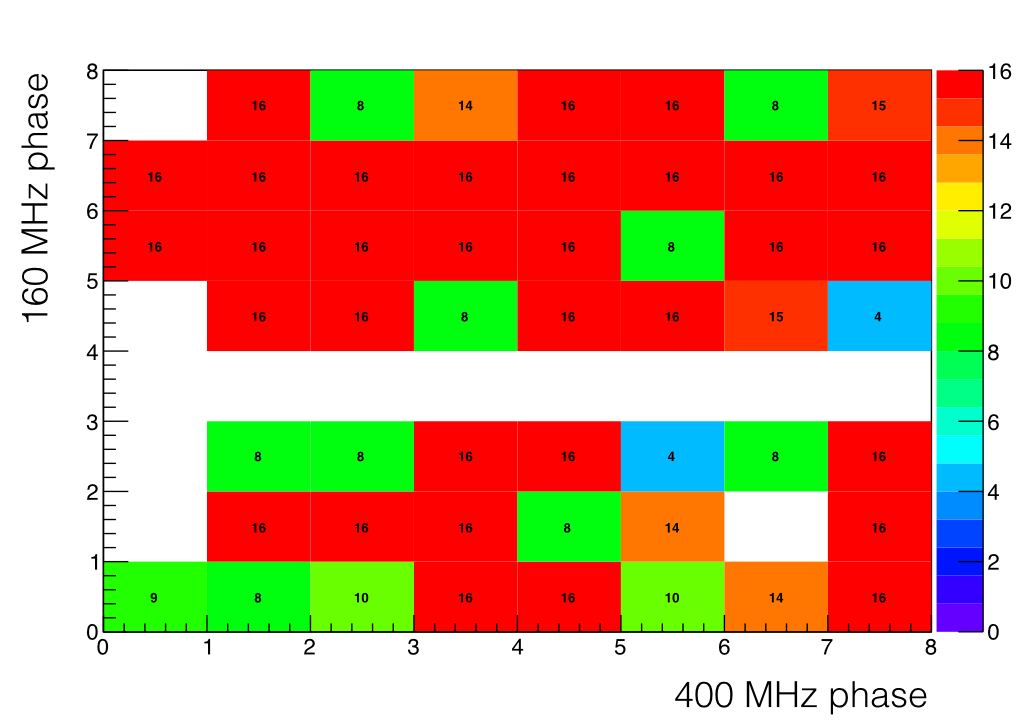
\includegraphics[width=0.45\textwidth]{\chsixteen/TMPLLDelayReadbackCalib.png}}
  \subfigure[]{\label{fig:TBMROCdelaysRB_b}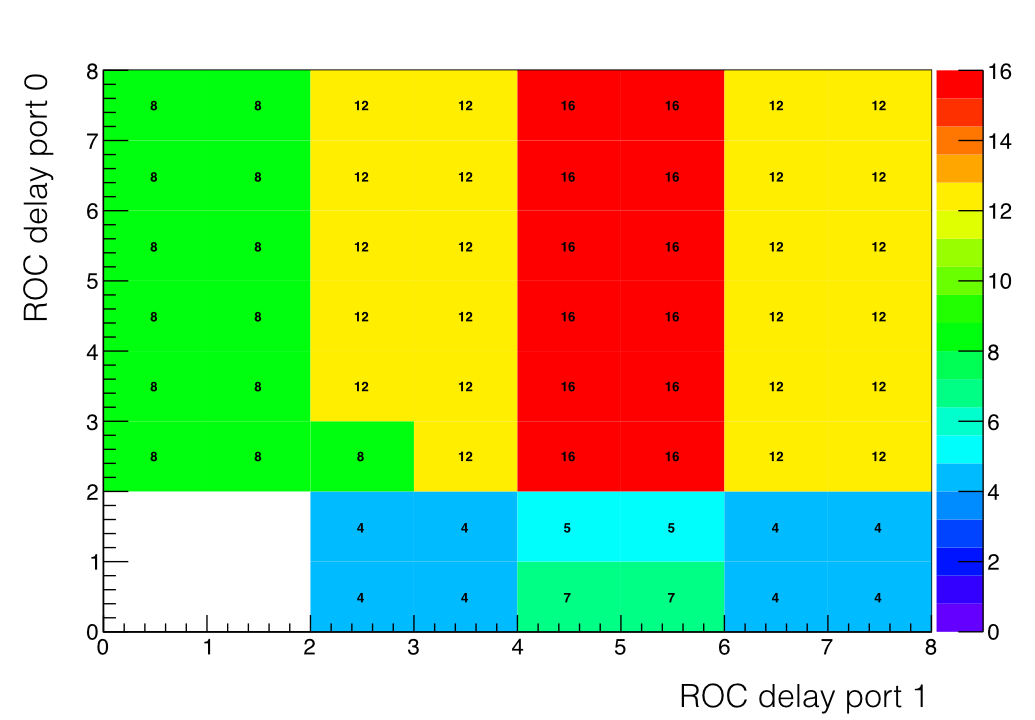
\includegraphics[width=0.45\textwidth]{\chsixteen/ROCDelayReadbackCalib.png}}
 \end{center}
 \caption{(a) Example of scan of the 2 TBM PLLs' phases (a) and ROC delays (b) for one module. For each pair of values it is verified that the message data obtained with the read back mechanism contain the expected ROC I$^2$C address. If the timing is correct, 16 ROCs per module have to be correctly identified.}
 \label{fig:TBMROCdelaysRB}
\end{figure} 

\subsection{ROC analog current and digital voltage}

The read back mechanism described in the previous section allows to assess the ROC analog current information ($I_{ana}$).
For the present detector it is possible to access only the total current of a large number of ROCs provided by a reading of the power supply, so that only an average value per ROC can be obtained.
As discussed in Chapter~\ref{ch:BPixCalib}, the analog current increases with irradiation and a re-calibration of the ROC analog voltage setting $V_{ana}$
is necessary to bring back the current in the safe range and recover the optimal ROC performance (Fig.~\ref{fig:PixRadDamag_b}).
The $V_{ana}$ calibration for each ROC is a time consuming procedure that converges after a large number of iterations of the S-curve test,
that allows for a measurement of the threshold every time the settings have been changed (Section~\ref{subsec:calibPart2}).
A much more simple procedure has been developed for the upgraded ROCs, since the measurement of the analog current is directly provided in the read back data.
The value is returned in ADC units and a conversion curve measured per each ROC during module testing is applied to obtain the corresponding value in mA.
The curve is of the form

\begin{equation}
I_{ana} (\mathrm{ADC}) = a + b \times I_{ana} (\mathrm{mA}) + c \times I_{ana}^2 (\mathrm{mA}),
\end{equation}

and its parameters are saved for each ROC in the detector configuration database.
As shown in Fig.~\ref{fig:ROCIanaCalib}, for each value of the $V_{ana}$ setting the analog current is readout from the ROC read back bits
and the conversion curve above applied to the original value in ADC.
At the end of the scan, a $V_{ana}$ setting corresponding to the target $I_{ana}$ value of 25\unit{mA} is chosen.

The same calibration code can be also configured to perform a measurement of the digital voltage $V_d$ per each ROC.
This parameter is controlled by a corresponding DAC and it is useful to monitor it as well during operations.
Its value can be returned by using the same read back mechanism but by changing the value written in the read back register.
As for the analog current, a ADC/mV conversion curve has been measured per each ROC during module testing
and it is applied in the final result of this measurement.

\begin{figure}[!htb]
 \begin{center}
  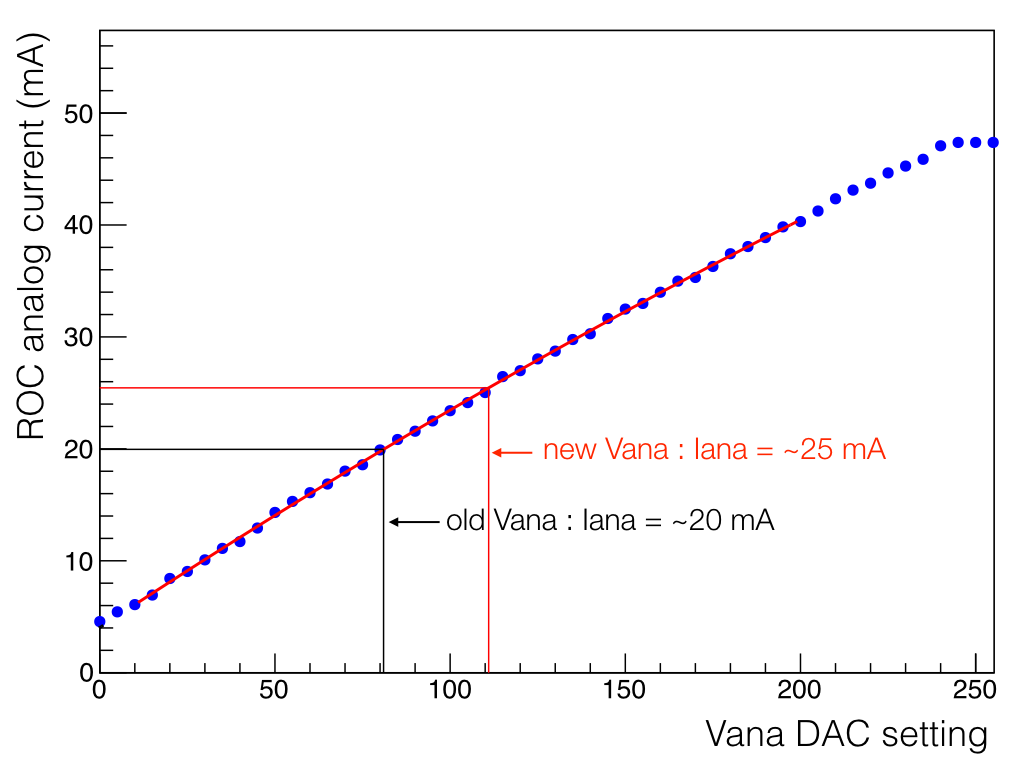
\includegraphics[width=0.5\textwidth]{\chsixteen/ROCIanaCalib.png}
  %\subfigure[]{\label{fig:ROCIanaCalib_b}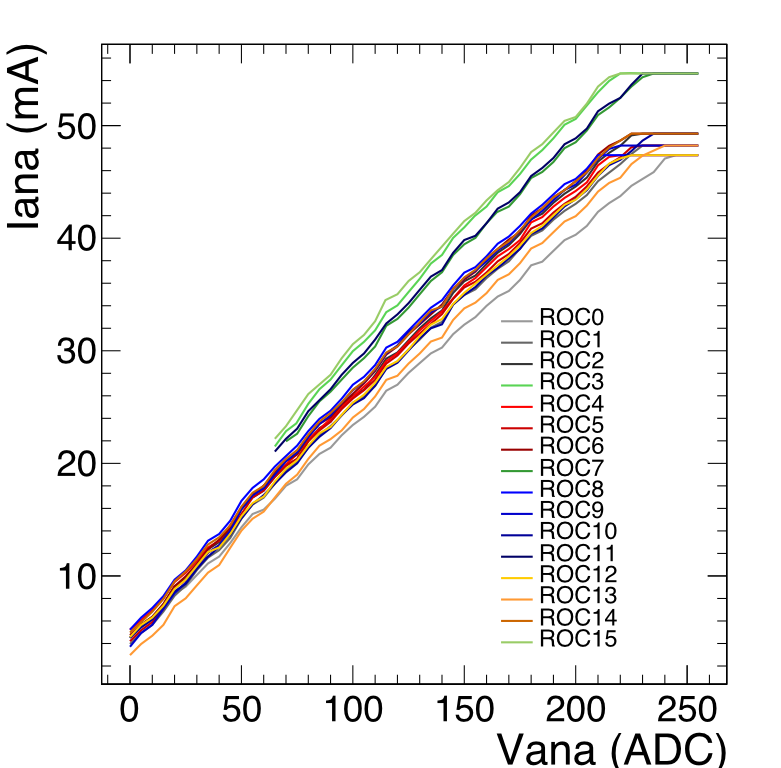
\includegraphics[width=0.39\textwidth]{\chsixteen/AllROCsIana.png}}
 \end{center}
 \caption{ROC analog current as readout with the ROC read back mechanism as a function of the analog voltage regulator setting.}
 \label{fig:ROCIanaCalib}
\end{figure} 

%\subsection{Other tests}
%\subsection{The test stand}
%\subsection{Detector commissioning}

